\documentclass[12pt, twoside, openright, a4paper]{gradient}
\usepackage{amsmath}
\usepackage{url}
\usepackage{acronym} 
\usepackage[english]{babel}
\usepackage{tikz}
\usepackage{amsmath}
\usepackage[colorlinks]{hyperref}
\usetikzlibrary{patterns}

% custom commands
\newcommand{\matr}[1]{\boldsymbol{\textbf{#1}}}
\newcommand{\wmatr}[1]{\matr{W}^{\text{#1}}}
\newcommand{\dd}[2]{\frac{\partial #1}{\partial #2}}
\newcommand{\vect}[2]{ \begin{pmatrix} #1 \\ #2 \end{pmatrix} }
\newcommand{\XT}{\matr{X}^{\text{T}}}
\newcommand{\XbI}{\vect{\matr{X}}{\beta \matr{I}}}
%\renewcommand{\vec}{\textbf}
\newcommand{\vt}[1]{\vec{#1}_t}
\DeclareUnicodeCharacter{2212}{\textendash}
\newcommand{\texthash}{\# }

% bibliography
\usepackage[backend=biber, citestyle=authoryear, bibencoding=utf-8]{biblatex}
\addbibresource{backmatter/bib.bib}




\graphicspath{{figures/}}

%% Til at tegne træer!
\usepackage{tikz}
\usetikzlibrary{positioning,arrows,calc}
\tikzset{
    on grid,
    node distance=3cm,
    auto,
    block/.style = {
        draw,
        shape=rectangle,
        minimum height=3em,
        minimum width=3em,
        line width=1pt
    },
    control/.style = {
        draw,
        shape=circle,
        minimum height=7em,
        minimum width=3em,
        line width=1pt
    },
    mux/.style = {
        draw,
        shape=rectangle,
        minimum height=1.5em,
        minimum width=1em,
        line width=1pt
    },
    empty/.style = {
        shape=rectangle,
        minimum height=3em,
        minimum width=3em
    },
    >=latex',
}


% code listings
\usepackage[scaled=0.6]{beramono}
\usepackage{minted}
\usemintedstyle{friendly}
\definecolor{bggrey}{rgb}{0.90, 0.90, 0.90}
\definecolor{bgwhite}{rgb}{1,1,1}
\setminted{bgcolor=bggrey, fontsize=\footnotesize, linenos, breaklines,obeytabs=true,tabsize=2,breaksymbolleft=}


% nice inline code
\makeatletter
\newcommand{\currentfontsize}{\fontsize{\f@size}{\f@baselineskip}\selectfont}
\makeatother
\setmintedinline{fontsize=\currentfontsize, bgcolor=bgwhite}
\newcommand{\ttt}[1]{\texttt{#1}}

\usepackage{listings}
\lstset{showspaces=false,
    showtabs=false,
    breaklines=true,
    showstringspaces=false,
    breakatwhitespace=true,
    escapeinside={(@}{@)},
    postbreak=\mbox{\textcolor{red}{$\hookrightarrow$}\space},
    %commentstyle=\color{greencomments},
    % keywordstyle=\color{bluekeywords}\bfseries,
    % stringstyle=\color{redstrings},
    basicstyle=\footnotesize \ttfamily,
    %numbers= false,
    frame=tb
}


% links in document
\usepackage{hyperref}
\renewcommand\UrlFont{\ttfamily\itshape}
\definecolor{linkblue}{rgb}{0.3, 0.3, 0.3}
\hypersetup{
  colorlinks=true,
  linkbordercolor=linkblue,
  pdfborderstyle={/S/U/W 1},
  linkcolor=linkblue,
  urlcolor=linkblue,
  allcolors=linkblue,
}

% show subsections in table
\setcounter{tocdepth}{2}



\usepackage[acronym,toc,shortcuts]{glossaries}
\makeglossaries


\begin{document}

\assignment{Master Thesis}
\author{Amira Moussa\\ \today}
\title{Acceleration of machine learning \\ 
through an FPGA}
\subtitle{A way to obtain minimal latency }
\frontpageimage{Cover/h.png}
\advisor{Asst. Professor Kenneth Skovhede}
\institution{University of Copenhagen}
\department{Niels Bohr Institute}

\maketitle
\frontmatter
\pagestyle{ruledtitle}
\begin{vplace}[0.5]
\section*{Acknowledgements}%
\label{sec:acknowledgements}

I want to express my gratitude to the {\em eScience} group that I was allowed to be a part of. Also, I am very grateful for Asst. Prof {\em Kenneth Skovhede} provided an open environment where I felt heard and supported. Further, I want to thank the members of the SME group who were always available to answer all of my questions, give me their feedback and inspire me during my time in the group. 
\\

Mainly, I want to thank {\em Carl-Johannes Johnsen} for the strong support during the work of my thesis. Without his insight, help, and encouragement, the goal of this project would not have been fulfilled.\\

Finally, I want to {\em thank Nam Tran} for being a great support throughout my studies and all of my friends who have read this thesis and made suggestions for improvements. Additionally, thanks to {\em Niklas Heim} and {\em Fabian Dornhecker} for letting me use this visually appealing template. 

\end{vplace}

\cleardoublepage
\section*{Abstract}%
\label{sec:abstract}
This thesis presents the design of an application
specific hardware for machine learning, which can be used in various physics applications, such as high energy physics and quantum optics.
Even though we are better at optimizing and have more computational power than ever, there is also a continuous need to make simulations even faster, more reliable, and cheaper to run. We are explicitly investigating a FeedForward Neural Network that interprets market data and enables minimal
round-trip times for executing electronic stock trades. There are similar trades, such as hard time restriction, which is also the case for computational physics. \\
This thesis optimizes the network to achieve the lowest possible latency. For this purpose, we use Synchronous Message Exchange \acrshort{SME} which is suitable for describing hardware and enables the flexibility to support a wide range of applied trading protocols. This demonstrates how to construct the components of a FeedForward machine learning script down to a processor as SME processes and how to connect them by
using SME busses. The complete system has been implemented in C\# and evaluated on an \acrshort{FPGA}. The results are promising compared to the Python implementation of the model. We present a proof
of the concept of an initial solution and its performance provides
results that make us believe that an entire Neural Network 
implementation would be feasible and competitive.
The final result is a successful implementation of a FeedForward Neural Network model on an FPGA, which runs 21 times faster than the same algorithm on a CPU.\\



\clearpage

\newacronym{HFT}{HFT}{High frequency trading}
\newacronym{SME}{SME}{Synchronous Message Exchange}
\newacronym{NN}{NN}{Neural Network}
\newacronym{FNN}{FNN}{Feedforward Neural Network}
\newacronym{GPU}{GPU}{Graphic Processing Unit}
\newacronym{CPU}{CPU}{Central processing unit}
\newacronym{ASIC}{ASIC}{Application-specific integrated circuit}
\newacronym{CSP}{CSP}{Communicating Sequential Processes}
\newacronym{Fintech}{Fintech}{Financial technology}
\newacronym{ML}{ML}{Machine learning}
\newacronym{HLS}{HLS}{High-Level Synthesis}
\newacronym{IP}{IP}{Intellectual Property}
\newacronym{FPGA}{FPGA}{Field Programmable Gate Array}
\newacronym{VHDL}{VHDL}{VHSIC Hardware Description Language}
\newacronym{BRAM}{BRAM}{Block ram}
\newacronym{CLB}{CLB}{configurable logic blocks }
\newacronym{CSV}{CSV}{Comma-Separated Values}
\newacronym{HDL}{HDL}{Hardware Description Language}
\newacronym{VHDL}{VHDL}{Very High Speed Integrated Circuit HDL}
\newacronym{ReLU}{ReLU}{Rectified Linear Units}
\newacronym{PReLU}{PReLU}{Parametic Rectified Linear Units}
\newacronym{GD}{GD}{Gradient Descent}
\newacronym{SN}{SN}{Shared-nothing Architecture}



\section{Notation}
In this project we highlight processes from the SME program with \texttt{this font}.\\






\printglossary[type=\acronymtype, title= Acronyms]
\begin{KeepFromToc}
\hypersetup{linkcolor=black}
\newpage\tableofcontents
\hypersetup{linkcolor=linkblue}
\end{KeepFromToc}

\mainmatter
\chapter{Introduction}
\label{cha:introduction}
\epigraph{
  \hypersetup{linkcolor=bgwhite}
  This thesis will investigate machine learning methods and examine or propose techniques for implementing them effectively in hardware. To validate and drive the design decisions, we will use a sample of applications from High-Frequency Trading \acrshort{HFT}, which has strict latency requirements. To avoid complexities in an already complicated implementation problem, we use a simple real-world feed-forward network for stock-price prediction obtained from an industry collaboration with a company wishing to remain anonymous and thus will not be mentioned.
  
  
 \iffalse
 Currently, the most commonly used hardware is the \acrshort{CPU}/\acrshort{GPU} because of their ease of use with high-level languages. However, by utilizing a Field-programmable gate array \acrshort{FPGA}, we could optimize time and energy since they possess the advantages of customized parallelism and design. The resulting plan will give us greater insight into reducing the latency of machine learning algorithms when implemented on an FPGA. This has implications for several real-world applications, including on-sensor evaluation of data in high bandwidth experiments, such as neutron accelerators and free-electron lasers. To validate and drive the design decisions, we will use a sample of applications from High-Frequency Trading, which has strict latency requirements.
 \fi
 
FPGAs are used in various physics applications, such as high energy physics and quantum optics, because of their versatility, programmability, high bandwidth communication
interfaces and signal processing capabilities.

Due to the complexity of programming, their use has been limited to somewhat simple applications.
However, many experiments could benefit from having a machine learning model on the FPGA. This is currently done in top-tier facilities, such as CERN.
This thesis explores the implementation of machine learning models on FPGAs using SME to accelerate inference. 
 
  %these characteristics and about the significant benefits that high-frequency traders get from the integration of FPGA hardware into their digital systems.
  

This chapter introduces the motivation behind optimizing HFT  alongside descriptions of commonly used processor architectures. Because the FPGA chips are not instruction-based hardware and have to be built upon hardware level, there is a need for a tool to translate the algorithms down to the hardware. In this case, we will use Synchronous Message Exchange (SME) which will be introduced in Chapter~\ref{cha:SME}. We want to implement a \acrshort{FNN} used in high-frequency trading to see if we can optimize the speed and efficiency of this model. The FNN model will be introduced in Chapter~\ref{cha:Neural Network}. The implementation of the FNN from Python to SME and then down to the FPGA will be described in \ref{cha:implementation}.
  Lastly, in Chapter~\ref{cha:results} the testing of the implementation and results will be discussed.
 
  \hypersetup{linkcolor=linkblue}
}



%\section{Background}
\section{High Frequency Trading}
\textbf{High-Frequency Trading} \acrshort{HFT} is an automated trading platform that large investment banks, hedge funds, and institutional investors use to automate trading. It consists of algorithms that run through powerful computers to transact many orders at extremely high speeds.
Over the last couple of millenniums, new technologies have constantly been developed, and with the evolution of computers, financial markets also evolved. Manual labor is increasingly being automated through the use of algorithmic trading strategies [\cite{gianluca2017high}].
One example of strategic algorithm trading is liquidity-providing strategies, where high-frequency traders try to earn
the bid-ask spread, which represents the difference of what
buyers are willing to pay, and sellers are willing to accept for
trading stock. "High volatility and large bid-ask spreads can be
turned into profits for the high-frequency trader while in return
he provides liquidity to the market and lowers the bid-ask
spread for other participants, adopting the role of a market
maker" [\cite{leber2011high}].

These types of problems are studied in deep learning programming. Moreover, these algorithms can work at multiple time scales, but the most interesting one is high-frequency trades that execute in milliseconds or less. At this time scale, machines are needed because of their speed and can process more information efficiently.

\section{Motivation}
\label{sec:motivation}
The stock market is moving towards \acrshort{HFT} and micro-optimization, which has received a lot of attention during the past couple of years [\cite{agarwal2012high}], turning it into an increasingly important component of financial markets. 

The demand for storing big data and running algorithms faster has reached its limit with the commonly used hardware, mainly the \acrshort{CPU} and \acrshort{GPU}. Companies interested in optimizing their trading have grown an interest for the \acrshort{FPGA}. These have specific technical characteristics that enable them to execute certain trading algorithms much faster than traditional software solutions. 

HFT algorithms compete on two dimensions: Firstly, they receive large amounts of stock market pricing data every microsecond.
Secondly, they must be able to act extremely fast on the received data, as the profitability of the signals they observe results in latency.

The first point is crucial. High-frequency trading is all about speed and minimizing latency. The faster you can run trading strategies and algorithms for analyzing minute price changes and executing trade orders, the higher the probability of gaining the most profit. 
Secondly, keeping a large amount of data in memory will slow down the hardware. Therefore, algorithms must use only a minimal amount of data and parameters stored in fast access memory. \\
Artificial neural networks have become a necessary tool in almost any area handling data and help predict future ranges from \ac{Fintech} to physics because of their abilities to predict different outcomes from complex relationships between data. Nevertheless, due to extensive incoming data and the need for faster inference, looking into other alternatives to implementing algorithms has grown. The FPGA has shown significant improvement in both power consumption and performance on some specific tasks when compared to the GPU and could therefore be a potential candidate as an alternative to the other hardware [\cite{FPGA}]. However, the FPGA is not ideal for replacing all processors because of its customization cost. Nonetheless, due to its parallelism, it could help optimize the latency of memory sharing, which would mean a lot in the \acrshort{HFT} field. The latency of memory sharing is vital as the algorithms developed by trading firms are competing on the scale of nanoseconds. To investigate these trade-offs, this thesis will explore how implementing a Feedforward network on an FPGA could potentially enhance the performance and whether it is worth replacing parts of the traditional hardware solutions with an FPGA.


\iffalse
Artificial neural networks have especially gotten popular in the financial-technology (fin-tech) area to handle data and help predict future changes in the stock market. But due to massive incoming data and fast transactions, the interest in looking into other alternatives on implementing their algorithms has grown. However, the FPGA is not ideal for replacing all processors, but it could help optimize the latency of memory sharing due to its parallelism. In this thesis, we will implement a Feedforward network on an FPGA and look at the performance to see if it is worth replacing hardware parts.
\fi







\section{The different hardware}
%machine learning algorithms are being used more in the fin-tech to extract and process information from raw data. 
Due to the increasing popularity of using ML in fin-tech, there has been a race to use the fastest hardware to achieve rapid predictions and trading  [\cite{FPGAvsGPU}].
Thus, there is a growing demand for hardware platforms to compute such intensive machine learning algorithms. As deep learning has driven most advanced machine learning applications, it is regarded as the main comparison point.
Nowadays, there are several types of processors, although when discussing heavy calculations, the main ones are the Central Processing Units (CPU), Graphics Processing Unit (GPU), Application Specific Integrated Circuit(ASIC), and Field Programmable Gate Array (FPGA). 

To understand the main applications and differences underlying each processor, the following section will present a brief overview of the different hardware and how they compare.

\subsection{Central Processing Unit}
\acrshort{CPU} is a chip that executes a program based on a specified set of instructions in a sequential manner. These are optimal for single-process systems, where the code needs to be executed sequentially or linearly.
The internal hardware structure is defined by the CPU vendor and cannot be modified [\cite{5272532}]. As a result, CPUs are general purpose and can thus perform any function based on the software program that is uploaded onto them.\\

\subsection{Graphic Processing Unit}
\acrshort{GPU} is a chip that performs fast mathematical calculations, primarily for graphics. In the 1980s, they were only used to offload pictures from the CPU [\cite{GPUvsfpga}]. As we progressed, drawings became more advanced, triggering a concurrent evolution of advanced GPUs. An image is composed of thousands of pixels processed by hundreds to thousands of identical cores that are specifically designed to execute the same program in a parallel manner. Because of their highly efficient parallel functioning, GPUs are now used in a variety of different fields and applications such as vector and matrix mathematics, for which they render jobs faster than the CPU [\cite{GPUvsfpga}]. The benefit is that instruction-based hardware can be bought as a finished product. This means that you can write instructions for them in different high-level languages, making it much easier for software engineers to work with. 

\subsection{Application-Specific Integrated Circuit}

Application-Specific Integrated Circuit \acrshort{ASIC} are single-purpose chips, meaning that they can only execute commands for which they have been specifically designed. 
Hence, they cannot perform another function or execute different applications once programming is complete [\cite{asic}]. The logic function of ASIC uses hardware description languages such as Verilog or VHDL.
However, CPU, GPU, and FPGAs are all types of ASIC, their applications being a general-purpose central unit, graphics-oriented, or field programmable, respectively.

Since these chips are built for a singular purpose, they do not have to run through unnecessary circuits to run a function, allowing the power consumption of ASICs to be very minutely controlled and optimized. As a result, they are often more power-efficient compared to other alternatives.



\subsection{Field Programmable Gate Array}
\acrshort{FPGA}, is a chip optimized for being re-configurable hardware, as in the user 'programs' the hardware circuit. 
A bare FPGA consists of small chunks of configurable logic blocks \acrshort{CLB} which can be configured to perform different functions. It consists of various components such as transistor pairs, look-up tables (LUTs), flip flops (registers), and multiplexers.
The blocks are connected with electronic wiring that can be turned on and off [\cite{asic}]. The logic blocks can be thought of as separate modules which can operate in parallel. These can be controlled, and it is possible to hook these together by programming the interconnects to build something meaningful.
An FPGA can be reconfigured by programming the logic blocks and manipulating the internal state. This can also be done even after deployment, which makes them ideal for systems and devices that need frequent updates such as prototypes, networking products, and other electronic systems [\cite{FPGA}]. Writing instructions to the FPGA can mainly be done in low-level languages such as \acrshort{VHDL} or \acrshort{Verilog}. \\


\subsection{Comparison}
The FPGA has a different architecture from the GPU and CPU, although in some cases, it is possible to apply either one for similar tasks. FPGAs tend to have more flexible architectures as compared to GPUs and CPUs. The main difference is that the CPU/GPU is instruction-based hardware, which means one can access the hardware using higher-level language. In contrast, the FPGA needs to be accessed from lower-level languages such as VHDL or Verilog.
This difference can make FPGA more responsive and allows more dedicated special-purpose implementation desired by the developer, described in [\cite{FPGA_CPU}].
CPUs/GPUs, comparatively, are easier to use for software engineers than FPGAs as the development process for the latter tends to be much more knowledge extensive and complicated than for the former, which explains why modern GPUs are being applied across a multitude of fields [\cite{GPUvsfpga}]. 

One of the prime features and advantages of FPGAs is that the entire internal hardware can be reprogrammed and reconfigured as the user is permitted to determine the logic of each block in the system. Hence, they are much more flexible in their programming and customized according to the programmer’s needs. 

FPGA is compared to ASIC reconfigurable, whereas the latter is permanent. The FPGA has a more straightforward design flow due to the flexibility of the chip, whereas the ASICs entail more complex design flows, given their reliance on a permanent architecture. The ASIC design requires dedicated and more expensive tools. The FPGA is a low-power-consuming chip compared to the CPU/GPU. It is more power-intensive in comparison to ASIC, which is a known established solution for battery-operated products.
The following Chapter will introduce the software to deploy code on the FPGA.

\chapter{Synchronous Message Exchange}
\label{cha:SME}
\epigraph{
  \hypersetup{linkcolor=bgwhite}

Synchronous Message Exchange (SME) [\cite{johnsen2021sme}] is a programming model used to develop highly concurrent systems. 
To translate the FeedForward neural network to the FPGA, we will use this tool to make it possible. The ideal goal is to program on a high abstraction level using, e.g., Python or C\texthash without knowing and working too much with a low-level programming language such as Verilog or VHDL. 

%The purpose of this Chapter is to introduce SME and give the reader a better understanding of the logic behind SME and the design ideas applied in this thesis. Notably, the purpose is not to go into deep theoretical and technical detail but instead provide the necessary background knowledge to understand the proceeding discussions.


%This should be accessible for software engineers without thinking about the technical part.

This chapter aims to provide an introduction to SME and give the reader a better understanding of the logic and the design ideas applied in this thesis. Notably, the purpose is not to go into deep theoretical and technical detail but instead provide the necessary background knowledge to understand the proceeding discussions.
The structure of SME is also introduced; for a more detailed description of using SME in a design see Chapter \ref{cha:implementation}. A brief guide is attached in appendix \ref{appendix:Sme_guide} with an emphasis on a small example to use SME on a simple Sigmod function. This function will also be used in the project. 


 % Chapter~\ref{cha:anomaly_detection};  
  \hypersetup{linkcolor=linkblue}
}


\section{Concurrent systems}
As introduced in Chapter~\ref{cha:introduction}, the unique characteristic of the \acrshort{FPGA} is the fact that it can handle concurrent computing.
Concurrent computing is a form of computing providing a way to make effective use of parallel and distributed systems that perform many simultaneous tasks using a multiprocessor [\cite{concurrent}]. The benefit of a multiprocessor is the ability %, which would be the FPGA. 
To conduct several tasks simultaneously, which enhances the speed
and efficiency. The efficiency is
determined by the speed compared to the resources used
in designing and implementing the multiprocessor, which will be the FPGA for this thesis.
However, working with concurrent systems also means contemporary problems, such as memory sharing. It can create a non-deterministic problem of reading and writing the
same memory, resulting in unexpected behavior.
An example could be the act of printing out an aligned set of numbers to your console using more than one thread, which is an independent set of the values in a process.
If the code is executed multiple times, the order of numbers will vary between the
runs. This is due to the time dependence in the threads. Consequently, time is an essential factor when working with concurrent systems. 


\subsection{Communicating Sequential Processes}
Various attempts have been made to solve this problem. Communicating Sequential Processes (CSP) [\cite{CSP}] was one, first proposed In 1978, \textit{Communicating Sequential Processes}~ [\cite{hoare_communicating_1978}] to
solve exactly these issues, and with it, CSP was created.
CSP was introduced as a model to describe patterns in concurrent systems and communication between sequential processes running in parallel. Currently, CSP is a formal method for modeling concurrent systems described by algebra.
CSP is built on two simple ideas, 'processes' and 'channels.’ A process is an ordered sequence of operations. These processes do not share any memory; therefore, one
The process cannot access a specific value in another process, which would solve the memory problem.
The other is channels, where the processes communicate with each
other by passing information. A simple example thereof is depicted in Figure \ref{fig:AB}, illustrating process \textbf{A} passing a
value onto a channel, which process \textbf{B} takes as an input. Once the deal is passed through the channels,
process \textbf{A} will lose access to it. This creates a messaging framework that enforces strict synchrony between communicating processes. However, the asynchronous nature
of CSP became a problem for hardware models. 
This laid the foundation for the establishment of Synchronous Message Exchange \acrshort{SME}.\\

\begin{figure}
  \centering
    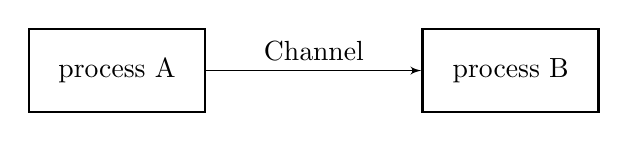
\begin{tikzpicture}[node distance=5cm,] 
        
        \node[block, text width=2cm, align=center] (sme) {process A};
        \node[block, right of=sme, text width=2cm, align=center] (ghdl) {process B};

        %connect
        \path[draw, ->] (sme) -- (ghdl) 
        node[midway,above, midway]{Channel};
        %\path[draw, ->] (ghdl) -- (sme);

    \end{tikzpicture}
    \caption{Communicating sequential processes from A to B }
    \label{fig:AB}
\end{figure}


SME was first introduced in 2014 and, after several iterations, has evolved to a programming model, a simulation library, and VHDL code generators [\cite{vinter2014synchronous}]. The original idea was conceived following an attempt to create a hardware implementation of a vector processor, modeled in PyCSP [\cite{CSP}], which is a CSP library for Python. The work was initially presented in the paper \textit{BPU Simulator}[\cite{Rehr13}], which introduced a high abstraction level simulation. The subject was explored more in detail in the master's thesis project [\cite{skaarup2014generation}], where two students implemented a vector processor using PyCSP. The results of this master's thesis made it clear that PyCSP could be used to model hardware: Nevertheless, this led to the discovery of different challenges, and CSP was therefore not sufficient.
Each process would have to read the clock signal to comply with the clock. To avoid race conditions, the
The system had to be implemented with a two-way clock.
This meant that the need to enforce global synchrony to the circuit resulted in an outburst. Even simple circuits became overwhelmingly large, as shown in Figure \ref{fig:csp}. Using PyCSP to model synchronous hardware would result in extensive and complex networks, which is not ideal for writing hardware models. This was because of the number of channels, which became enormous for controlling the progress and simulating the clock.
The conclusion was that PyCSP alone was not a viable tool for describing timed hardware since it is forcing a globally synchronous environment onto the
CSP model. A potential solution could be to isolate the processes and connect via channels, which has shown to be a better approach for building larger hardware models [\cite{vinter2014synchronous}].

\begin{figure}
  \centering
  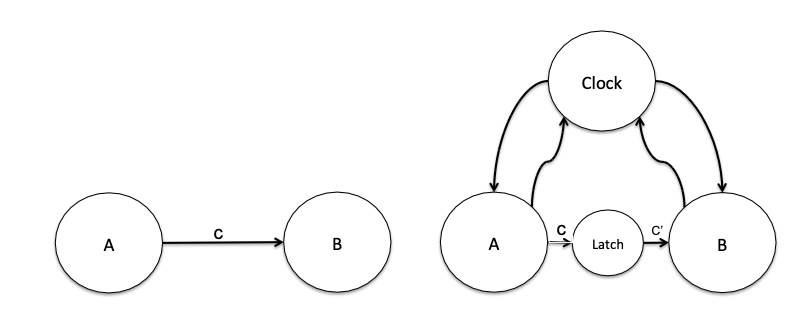
\includegraphics[width=0.7\linewidth]{Pictures/CSP.png}
  \caption{Enforcing global synchrony on a simple CSP model, where the channel \textbf{C} transfer information from the process \textbf{A} to process \textbf{B}, resulting in an increasing complexity. Figure from [\cite{vinter2014synchronous}]}
  \label{fig:csp}
\end{figure}

\section{Synchronous Message Exchange}
\label{sec:SME}

Most of this theory is based on [\cite{vinter2014synchronous}] and [\cite{SME2020}].
The motivation behind SMEs rose from the need to provide a simple framework for programming an FPGA.
It is an environment for developing and testing hardware designs for FPGAs in C\#. With SME, it is possible to create hardware structures translated to VHDL. 
However, FPGAs can be a better choice for energy-sensitive applications since FPGAs can, in some cases, achieve the same performance as a GPU but with lower energy consumption [\cite{SME2020}].
Previously, the developer needed to design an integrated circuit on the gate level for the FPGA. This could be difficult due to the low-level languages' design framework, which is not common knowledge amongst software developers. Some high-level methods for programming an FPGA have been developed. However, these are often tedious to work with. Thus, designing and implementing hardware models is beneficial with SME.\\

The goal with SME is to give software developers a tool that provides the opportunity to program hardware but with an added abstraction layer that separates the developer from the hardware details. The development resembles the structures and semantics known from software development.


The idea is to develop individual processes, test them through simulations and then connect them to larger hardware models. Leveraging the features of a modern $C\#$ Integrated Development Environment, such as Visual Studio, makes it much faster to develop, experiment, and test FPGA designs, especially for a software developer. SMEs add a software abstraction layer that conceals the complexity typically requiring high-level FPGA expertise.
SME was built on the requirements of a
\textbf{Hidden clock }, 
\textbf{Global synchronization}, 
\textbf{Broadcasting channels (Busses)}, 
\textbf{Shared nothing } and 
\textbf{Implicit latches }.\\


\subsection{The hidden clock and global synchronization}
Many factors have to be considered when writing in hardware, such as timing. Since processes could read and write signals, there is no way of knowing if the following processes would use old or new data. Therefore, some predictability for the hardware is required, so global synchronization is needed.
The hidden clock is made to establish coordination between processes by synchronizing them all. An SME model consists of clock cycles and one hidden clock that is then propagated out to all the processes having a clock cycle and activates them.
A clock cycle is a period between each signal, divided by all processes.
An SME clock cycle consists of three phases: reading, computing, and writing. The visual explanation could be shown as a step function going from high to low, see Figure \ref{fig:clock}, The process is activated on the rising clock when the process is executed where it reads from the bus, and then it computes and writes to the bus, all in one clock
cycle. Just before the rising edge of the clock, all signals are propagated on all busses, which means that all communication happens simultaneously.
Un-clocked processes will first be activated when the input has been written to by other methods processes.

\begin{figure}
  \centering
  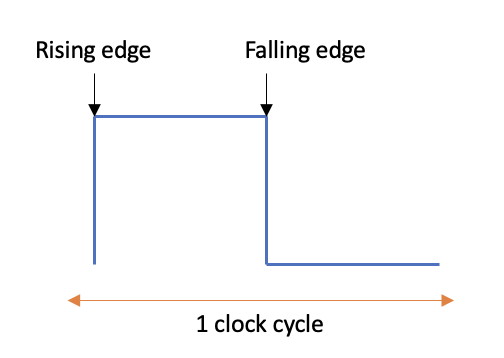
\includegraphics[width=0.5\linewidth]{Pictures/clockcycle.png}
  \caption{Illustration of a clock cycle}
  \label{fig:clock}
\end{figure}

The SME model supports both synchronous and asynchronous processes, whereby synchronous processes run during every clock cycle. In contrast, an asynchronous process is only run when receiving all of the signals on its input buses. 



\subsection{Broadcasting and busses}
In CSP, processes communicate with each other using channels that use the rendezvous protocol, meaning that data gets transmitted through the channel once the destination says it is ready to receive and vice versa.
On the contrary, SMEs use broadcasting channels called busses, from which any process can be read. This means that a process can broadcast its output to multiple processes through a single bus. Using CSP, multiple channels would have to emulate a single bus in SME. The busses define and manage the data that is exchanged between processes. These can be visualized as a pipe or a channel. When data is written to a bus it
will be available in the following clock cycle if it is a clocked process and available right
away for un-clocked processes. Furthermore, a bus can contain multiple data types and values that a process can access. 

\begin{figure}[H]
  \centering
  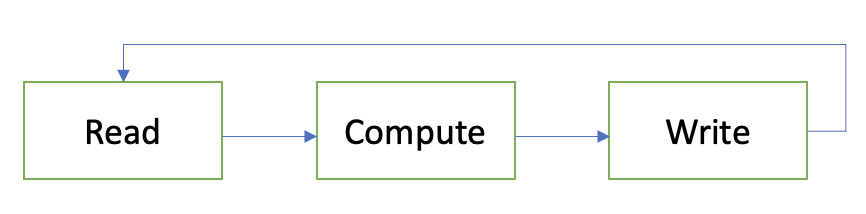
\includegraphics[width=0.7\linewidth]{Pictures/readbus.png}
  \caption{SME process for one clock cycle.}
  \label{fig:readbus}
\end{figure}


\subsection{Shared nothing}
The fastest way to handle data through hardware is by addressing memory separately.
A \acrshort{SN} is a distributed computing architecture in which you have several separate nodes that do not share memory or storage.
Operating under numerous self-sufficient nodes rather than having a single source of particular resources offers several advantages: easier scaling, non-disruptive upgrades, eliminating a single point of failure, and self-healing capabilities.
SN eliminates single points of failure, allowing the overall system to continue operating despite losses in individual nodes and allowing individual nodes to upgrade without a system-wide shutdown [\cite{sharednothing}]. 

\newpage


\section{Hardware Description Language}
Generally, implementing code down to \acrshort{FPGA} is programmed using Very High-Speed Integrated Circuit HDL \acrshort{VHDL}. This is harder to use since it is intended primarily to be a parallel programming language. This can be challenging, especially for a software engineer implementing an FPGA.
The vendors are not implementing recent updates to VHDL, and so it is not evolving with time or the programmer [\cite{SME2020}]. \\

The SME framework is implemented in the .NET framework, the version of SME that will be used throughout this thesis.
With the C\# SME library, it is possible to write all control logic in C\#.
All data written to a bus can be logged for each clock cycle and saved as a test bench, a piece of software used for
testing hardware models. It provides input data to the hardware model and verifies its output which is saved as a \acrshort{CSV}. Hence, it can then be used for compiling the program into VHDL, which can be put onto FPGA circuits. This eliminates the need to write a separate VHDL test bench, which immensely improves developer productivity. This is needed since some of the implementations are still manually done to implement on hardware, which will be in Vivado. A further explanation of the performance can be found in Chapter~\ref{cha:implementation}.




\section{SME setup and structure}

To show the basic structure of how SMEs works, we will go over the fundamental design. For further explanation on how the system was set up for the whole project, see Chapter \ref{cha:implementation}.
When analyzing the general structure of our SME program, there are three main structures:
\begin{enumerate}
    \item \textbf{Connection}: How the circuit is connected, i.e., which busses connect to which processes.
    \item \textbf{Processes}: The process structure for each function and how they behave.
    \item \textbf{Verification data}: All data from the Python FNN that could be useful for the verification of the hardware model.
\end{enumerate}



\subsection{Connection}

The fundamental structure behind the SME network is the communication between the processes through busses. Understanding different communication structures in SMEs will provide the insight necessary for designing the translated systems of the Python model.
A network in an SME program is a crucial part that connects all processes with
communication. Defining the network from process instances
also has the advantage that one process can be instantiated with different parameters several
times within the same network, providing the possibility of reusing the processes for different
purposes.

\subsubsection{Busses}
As previously explained, an SME bus defines a collection of channels used for all
communication between the processes. Each channel has a type describing the communicated
data and can be initialized with an initial value. The IBus interface marks an interface as a bus of a read or writes in SME, which is shown as an example in Listing \ref{lst:bus} where we define a \emph{bus} to transfer a value. 
An SME bus has an identifier used for referencing the bus. All channels within a bus are connected to the process simultaneously, and it is up to the developer to call the correct channel within the bus for either a read or a write. 

\begin{listing}
  \inputminted{csharp}{codesnippets/bus_value.cs}
  \caption{Simple bus that transfers one value}
  \label{lst:bus}
\end{listing}


\iffalse
\begin{listing}
  \inputminted{csharp}{codesnippets/bus_example.cs}
  \caption{bus that transfers an index and is set to with a Boolean}
  \label{lst:bus_example}
\end{listing}
\fi

\subsection{Process structure}
The processes in an SME program describe the fundamental behavior of a model.
An SME process is defined by the \emph{SimpleProcess} class and consists of an identifier, process parameters, bus, and variable declarations. The body of the process, the process statements, consists
of sequential notices such as communications and calculations to be evaluated once
for each clock cycle. 
%A small example of an SME process has been presented in Appendix \ref{appendix:Sme_guide}.

A process is initiated in the network of an SME program. A process can be instantiated with a set of parameters. These parameters can
be a mix of input and output busses and constants.

When defining a process, we can give either an \textbf{Input Bus} or a \textbf{Output Bus}.
The name of the input bus can be given as a process parameter, which the process can use to read from the actual bus channel, as can be seen in App. \ref{appendix:Sme_guide} Listing \ref{lst:sigmoidSME}. In this example, the process reads the data from \emph{m\_input} in the bus and writes the data to the \emph{m\_output}.




\subsection{Verification data}
It will always be necessary to generate input for pure SME networks, which can be done in multiple ways. One way of initializing the SME network data is by giving the process a constant given as a parameter or by hard-coding internal values into the process. Another way is to have a separate process that generates data for the network. The first attempt to write a process to generate data is shown in the example App. \ref{appendix:Sme_guide} Listing \ref{lst:sigsimulator}.
Here the process clock is a data generating process. It does not read data from any input bus. Thus, it can only create data to write to the network. The example shows the \texttt{Sigsimulator} which generates values from $[1,10]$ and writes it out onto the output bus. A further explanation of the structure of a process will be introduced further in Chapter \ref{cha:implementation}.
Another way to generate data is to make a process that imports the data and reads them through a bus. This was created as a simple SME process structure, where the function reads the data from a CSV file and saves it as a flat array. This is shown in Listing \ref{lst:datagenerator}.

An SME process that does not read any input is just a data generation process, but in this case, we use the input bus \emph{index} to make sure that each value that reads from the CSV file gets an index.
The output-bus transfers the array of data and makes sure it gets written out.
In \ref{lst:datagenerator} the \emph{async process} only runs when the index is ready.  The address will save each value and write them out in an array.


\begin{listing}
  \inputminted{csharp}{codesnippets/datagenerator.cs}
  \caption{C\# code to import an \emph{input} CSV file, using SME processes to save the data \emph{output} as a flat array}
  \label{lst:datagenerator}
\end{listing}

\newpage


\section{Related work}
As mentioned in Chapter \ref{cha:introduction}, FPGAs contain many exciting properties, which makes them more flexible to use, faster, and more energy-efficient than GPU/CPUs for specific tasks. Algorithms are getting more complex and energy-consuming.
FPGAs are not widespread due to the low-level language used to program the chip [\cite{fang2020memory}]. This has started a minor movement in building alternative implementation frames such as SME.
An exciting framework constructed from the same idea is \textbf{hls4ml}, which was made as a joint project between Xilinx and CERN for accelerating the inference of processing data [\cite{hls4ml}]. A growing team of physicists and engineers from CERN wanted to have a flexible way to optimize custom event filters in the Compact Muon Solenoid (CMS) detector they are working with at CERN. The very high data rates in the CMS detector required event processing in real-time, but trigger filter algorithm development hindered the team’s ability to make progress [\cite{fahim2021hls4ml}].
hls4ml is built on the idea of being a user-friendly software based on High-Level Synthesis (HLS), designed to deploy network architectures on FPGAs. This is done in $C$ as a sequential programming model designed for CPUs rather than FPGAs. As such, it is not uncomplicated to gain performance, as it relies on automatic derivation of parallelism.
Among others to describe hardware using higher-level language are \textbf{Chisel-lang} [\cite{chisel-lang}], which is similar to SME but described as a library in Scala. This means that the programmer needs to be able to keep two states of the program in mind, one that is running in Scala, evaluating some specific condition statements, and another running the generated code, not being able to see the condition statements [\cite{SME2020}].
\textbf{OpenCL }is a popular framework that intent to get more GPU programmers on board.[\cite{OpenCL}]
However, the focus here is not to accelerate with FPGAs, and as introduced in chapter \ref{cha:introduction}, the different hardware has different benefits.
And \textbf{QuokkaEvaluation} [\cite{QuokkaEvaluation}] is still an ongoing project focusing on specific FPGA implementations and has similar elements from SME, but is still in the initial phase.


\chapter{FeedForward Neural Networks}
\label{cha:Neural Network}
\epigraph{
  \hypersetup{linkcolor=bgwhite}
Neural Networks are a set of models inspired by the human brain that can be used to recognize patterns by finding regularities and similarities in data using machine learning data [\cite{patterns}]. The word Neural originates in the
McCulloch-Pitts neuron [\cite{Mcculloch}], a simplified model of the
human neuron as a kind of computing element that could be described in terms of
propositional logic. Just like the
brain, Neural Networks are constructed from small neurons or perceptrons connected with weights. These are made to process and pass on incoming data. The patterns they recognize are numerical, contained in vectors, into which all real-world data, be it images, sound, text, or time series, must be translated first [\cite{Goodfellow-et-al-2016}]. \\

In this chapter, we introduce the basic principles behind a Neural Network.
This will be followed up by the architecture of a FeedForward Neural Network \acrshortrshort{FNN} where the computation proceeds iteratively from one layer of units to the next. This will come in handy for the implementation.  \\
This section’s general introduction to the architecture of FeedForward Neural Networks is mainly based on the books [\cite{Jurafsky2009}] and [\cite{Goodfellow-et-al-2016}]. 



 % Chapter~\ref{cha:anomaly_detection};  
  \hypersetup{linkcolor=linkblue}
}
 

\section{Artificial Neural Networks}
\label{sec:FeedForward}

\begin{figure}
  \centering
  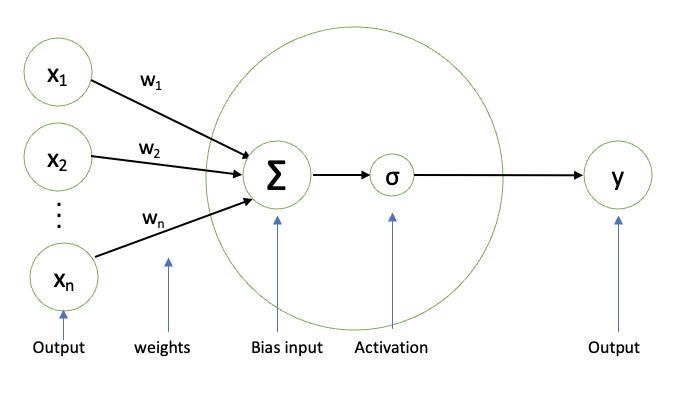
\includegraphics[width=0.7\linewidth]{Pictures/neuron.png}
  \caption{Single neuron model where the neurons $x_i$ takes the n weighted inputs plus a bias. This is an example for a linear case given to the activation function which then outputs an $y$ } 
  \label{fig:perceptron}
\end{figure}

Machine learning is a form of applied statistics focusing on using computers to estimate statistically complicated functions. By having a data set, the goal is to find a function that fits a data set best. One class of modeling is Neural Networks which have been shown to work well. One way to use Neural Network is by applying \acrshortrshort{FNN}.\\
But first consider the mathematical model shown in Figure \ref{fig:perceptron}. This is the simplest example, and the building block of a Neural Network called a single computational unit or a perceptron. A unit takes
a set of real-valued numbers as input, computes them, and produces an output.

More specifically, a Neural unit takes its inputs $x_i$ and their weighted sum $w_i$, which determines the contribution of a given input to the output, with one additional term in the sum called a bias term $b$.
The weighted sum $z$ can be represented as:
\begin{equation}
  \label{eq:ffn_eq}
  z = \sum_i^n w_i x_i + b
\end{equation}
The sum over all the inputs multiplied by their weights can conveniently be represented by a dot product. 
\begin{equation}
  \label{eq:ffn_eq}
  z = w \cdot x + b
\end{equation}

\subsection{Activation functions}
Instead of using a linear function $z$ as the output, Neural units apply a non-linear function $f$ to $z$. This is called an activation function. 
The \emph{feed forward Neural Networks} (FNN) lets information flow through the function being evaluated from x, through the activation function $\sigma$, and finally to the output, $y$. Figure \ref{fig:perceptron} shows a schematic neuron where the unit goes into the activation function and gives the output y.
%shows a simple schematic of a single neuron.
%Since we are only modeling a single unit, the activation for the node is, in fact, the final output of the Network, which we’ll generally call $y$. 
The value $y$ is given by:
\begin{equation}
  \label{eq:activationfunc}
  y = \sigma(z) = \sigma(w\cdot  x + b)
\end{equation}

The bias $b$ measures how easy it is to activate the neuron. Generally, there are a great variety of functions. For this project, we will only discuss the three non-linear functions applied here - the Sigmoid, \acrshort{ReLU}, \acrshort{PReLU} and Softplus.\\

\textbf{Sigmoid}: The sigmoid function, which is shown in Figure~\ref{fig:sigmoid},
\begin{equation}
\label{eq:sigfunc}
  \sigma_{sig} (z) = \frac{1}{1 + e^{-z}},
\end{equation}
takes the real valued number and maps it to a value into the range $[0,1]$ which is useful because the outliers get squashed toward 0 or 1.

\begin{figure}
  \centering
  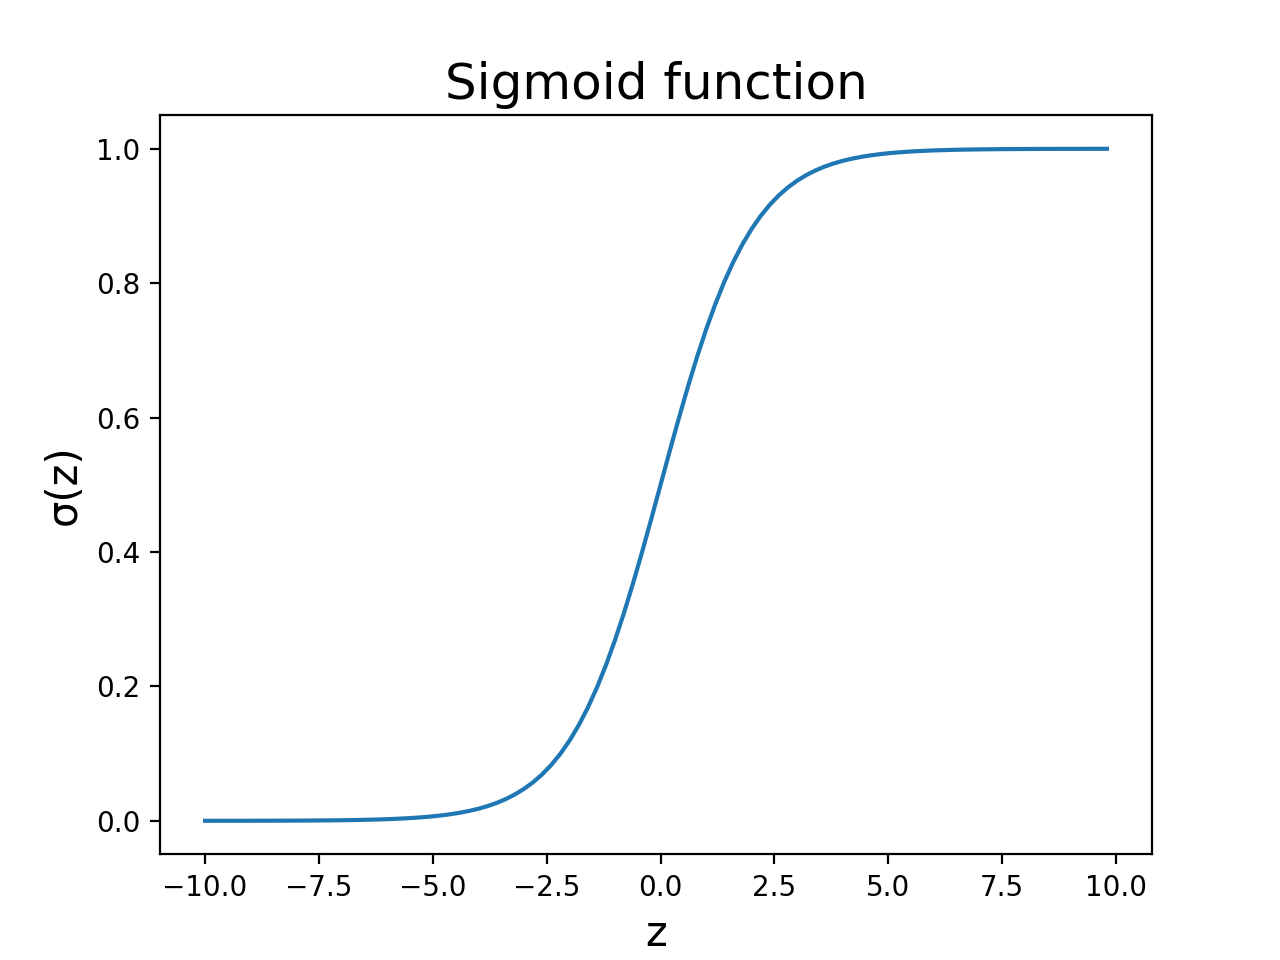
\includegraphics[width=0.5\linewidth]{Pictures/sig.PNG}
  \caption{Sigmoid Function. Frequently used as an activation function in FNN
  The sigmoid function takes a real value and maps it to the range [0,1]}
  \label{fig:sigmoid}
\end{figure}


substituting Eq.\ref{eq:activationfunc} into Eq.\ref{eq:sigfunc} 
gives the output 

\begin{equation}
\label{eq:sig_full}
  y = \sigma_{sig} (w\cdot  x + b) = \frac{1}{1 + exp(-(w\cdot  x + b))},
\end{equation}

\textbf{ReLU}: Rectified Linear Unit is the most commonly used activation function in deep learning models. The function returns 0 if it receives any negative input but returns that value for any positive value  x. So it can be written as

\begin{equation}
%\label{eq:sigfunc},
  y = \sigma_{PReLU} = \begin{cases} x & \text{for x > 0},   \\
        0.01 x & otherwise      %
        \end{cases}
\end{equation}


\textbf{PReLU}: Parametric PReLU (PReLU) makes it a parameter for the Neural Network to figure out itself: $y = \alpha x$ when $x < 0$, where $\alpha$ is a parameter and $x$ is the input. If $x \geq 0$ then $y = x$. 

\begin{equation}
%\label{eq:sigfunc},
  y = \sigma_{PReLU} = \begin{cases} x & \text{for x > 0},   \\
        \alpha x & otherwise      %
        \end{cases}
\end{equation}


PReLU is another popular activation function because it resolves an issue called "the dead neuron problem," which is familiar with the ReLU function. This problem occurs when inputs approach zero or are negative, which will make the gradient of the ReLU function
zero [\cite{QingJie_2017}]. This implies that with poor initialization, where most neurons have negative output, these
neurons will have no incentive to adjust their weights. Hence the Network will have limited ability to "learn.” PRelu addresses this issue, given that it doesn’t have zero-slope parts.\\


\textbf{SoftPlus}: Finally, the softplus function is a smooth approximation to the PReLU activation function and is sometimes used in the Neural Networks in place of PReLU. It is closely related to the sigmoid function. In particular, when $x \to$ −$\infty $, the two functions become identical.

\begin{equation}
\label{eq:softfunc}
 \sigma_{soft}= \log\left(1+\exp{x}\right),
\end{equation}

However, these activation functions have different properties, making them useful for different Network architectures. For example, the \acrshortrshort{ReLU} function has beneficial properties. Networks trained with the rectifier function almost completely avoid the problem of vanishing gradients, as the gradients remain proportional to the node activations [\cite{Goodfellow-et-al-2016}]. Contrary to the sigmoid function, containing exceptionally high values of $z$ result in values   of $y$ that are saturated, i.e.,
Extremely close to 1, which causes problems for learning [\cite{Jurafsky2009}]. Rectifiers don’t have this problem since the output of values close to 1 also approaches 1 in an excellent gentle linear way.

\subsection{The XOR problem}
\label{sec:xor_problem}
When sending data to a unit, it goes through the activation function, which reduces the sum of the input values to a 1 or 0 value, or at least a value very close to. If we consider the task of computing elementary logical functions of two inputs, like AND, OR, and XOR, we get the truth tables, as shown in Figure \ref{fig:truthtables}

\begin{figure}
  \centering
  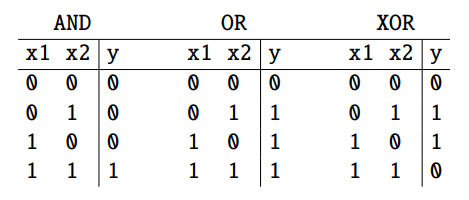
\includegraphics[width=0.5\linewidth]{Pictures/truthtable.PNG}
  \caption{Truth tables of elementary logical functions of two inputs for AND, OR and XOR. The XOR gives the output 1 if the inputs are different from each other and 0 if they are the same }
  \label{fig:truthtables}
\end{figure}

On the surface, this appears to be a simple problem. However, as shown by Minsky and Papert in 1969 [\cite{minsky69perceptrons}], this becomes an issue for a Neural Network that is only based on a single perceptron. The difference is that a perceptron is purely linear, and a unit is non-linear. If we look at a two-dimensional problem for the different truth-tables in Figure \ref{fig:xorgraph}, we see the possible logical inputs (00, 01, 10, and 11) and the line drawn
by one possible set of parameters for an AND and an OR classifier. 
If we look at the AND example we see, that when $x1=1$ and $x2=1$ then $y=1$ and in all other cases, it is 0, so if you wanted to separate all the ones from the zeros by drawing a single line, you would draw the line as shown in the graph.

\begin{figure}[h]
  \centering
  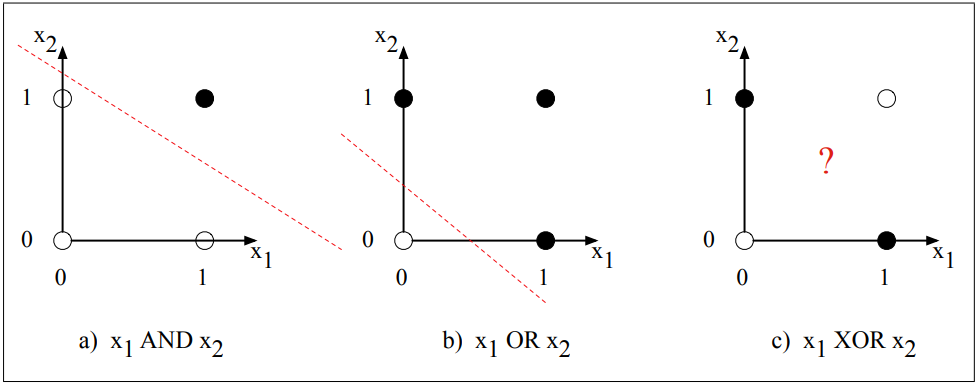
\includegraphics[width=0.7\linewidth]{Pictures/XORgraph.PNG}
  \caption{Truth-tables of elementary logical functions of two inputs for AND, OR and XOR [\cite{Jurafsky2009}]}
  \label{fig:xorgraph}
\end{figure}

A single line can separate this class. They are linearly separable patterns, meaning classes with an n-dimensional vector can be divided with a single decision surface.

That is how the perceptron works; it draws a boundary to separate the binary values. When the perceptron is trained, the value of the weights will be adjusted to form the line shown. Since the perceptron's output is a linear function, the two classes must be linearly separable for the perceptron Network to function correctly. 

Let’s see what happens with XOR problem that gives $y=1$ if $x_1\neq x_2 $ and  $y=0$ otherwise.
Notice that there is simply no way to draw a line that separates the positive cases of XOR (01 and 10) from the negative points (00 and 11). Hence, we conclude that XOR is not a linearly separable function.
Instead, we will have to draw multiple lines and thus require various perceptrons. In n-dimension, if you can draw a hyperplane to separate the binary values, you can use perceptrons to solve that problem.



\section{FeedForward Neural Network}
Having provided the necessary background knowledge behind units/perceptrons and how they work, next, we will need to elaborate on the functioning of the \textbf{FeedForward Neural Network or FNN}. A FeedForward Network consists of multiple layers in which the units are only connected in one way and
often applied to classification tasks, such as the recognition of a certain
shape in an image. There are three layers: the input, hidden, and output layers.  However, the characteristic and core of a \acrshortrshort{FNN} is the hidden layer, which consists of units described in \ref{eq:activationfunc}. The output of each layer is passed to teams in the hidden layer, which sums over all the input units until the final layer gives the final output. Figure \ref{fig:fnn_layers} shows an FNN where the input layer represents the data that is fed into the Network, followed by one or more hidden layers and an output layer.

We can think of a fully-connected Network as a function $F$ : $\mathbb{R}^n \to \mathbb{R}^m$ that maps the input $(x_1, .., x_n)$ to the output $(y_1, .., y_m)$ We
are now considering a structure of numerous neuron ordered in different layers. Therefore, $F$ can be split into a chain of simpler functions $f^{(i)}$, where  $f^{(i)}$ correspond to activation/output of the neurons in the i'th layer.

\begin{equation}
    F(x) = f^{(out)}(..f^{(i)}(..f^{(1)}(x)..)..),
\end{equation}

Where the first layer after the input layer is represented by $f^{(1)}$ and the final layer as $f^{(out)}$, the input layer is usually not counted when enumerating layers, but we call it the 0'th layer.

In a Neural Network, we only know the
input and the output from the final layer. The activation  $f^{(i)}$ of the layers in between is not shown, which is why
they are called hidden layers. A network consisting of more than one hidden layer is called \emph{deep Neural Network}, where we define the model depth as the number of hidden layers in the Network, thus, not counting the input and output layer. 
It is common for hidden layers to be much larger than
the input and output layer in deep Neural Networks because having larger dimensions give the best prediction [\cite{Goodfellow-et-al-2016}].  The number of weights for deep
Therefore, networks become approximately proportional to the square of the count of
nodes per layer in these largely hidden layers. Instead, we can think of layers as we described the neurons. Now just with a bias $b$ as a vector and the weight as a matrix $W$, consisting
of the combination of the weight vector $w_i$ and bias $b_i$ for each unit $i$. From a visual point of view as illustrated in Figure \ref{fig:fnn_layers}, we can represent each element of matrix $W$ as $W_{ji}$ where it connects the   $i$th input $x_i$ unit to the $j$th hidden unit $h_j$. By representing it with a single weight matrix $W$, the output of the hidden layer $h$ is thus:

\begin{equation}
  h = \sigma(W x + b)
  \label{eq:hidden_layer}
\end{equation}

where $\sigma$ is applied to a vector elementwise, so $\sigma[z_1,z_2,z_3] = [\sigma z_1,\sigma z_2, \sigma z_3]$.

The dimensionalities of these vectors
and matrices are enumerated as $n_0, n_1$ and $n_2$ for respectively the input, hidden and output layer. Here $x \in \mathbb{R}^{n_0}$, $h \in \mathbb{R}^{n_1}$ and $b \in \mathbb{R}^{n_1}$, since each hidden layer can take a different bias. The weight matrix therefor has dimensionality $W \in \mathbb{R}^{n_1 x n_0}$.

The matrix multiplication from equation~\ref{eq:hidden_layer} is thus:

\begin{equation}
    \begin{split}
  h & = \sigma \left(\sum^{n_0}_{i =1}  W_{ji} * x_i  + b_j\right) \\
  &= f^{(i)} = \sigma (W^{(i)} *  f^{(i-1)}  + b^{(i)})
    \end{split}
\end{equation}

\begin{figure}
  \centering
  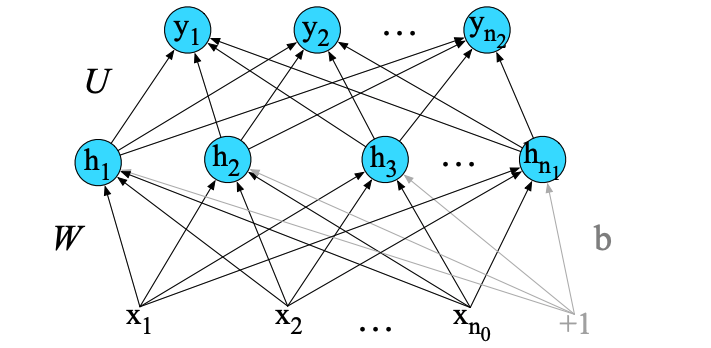
\includegraphics[width=0.7\linewidth]{Pictures/fnn_layers.png}
  \caption{A simple FeedForward Network, with one input layer (not counted as layer), hidden layer and one output layer [\cite{Jurafsky2009}]. }
  \label{fig:fnn_layers}
\end{figure}



where $f^{(i-1)}$ is the output from the $(i-1)^{th}$ layer.
Like the hidden layer, the output layer also has a weight matrix $U$ and sometimes a bias, but we will look at a simple example without the bias for simplicity’s sake.
The weight matrix for the output layer is multiplied by its input vector from the layer before, which is the hidden layer $h$, to produce the intermediate output z.

The output of the hidden layer $h$ is thus:
\begin{equation}
  z = U h
\end{equation}

Since z is a vector of real-valued numbers and needs a classification of probabilities, we can use a normalization function such as the softmax to get a probability distribution.
The output of the hidden layer $h$ is thus:
\begin{equation}
  y = \text{softmax}(z)
\end{equation}

In this way, the layers in FNNs can model arbitrary functions and separate data sets that are not linearly separable. This linearity is only broken by the activation function contained in the hidden layers, which act as a non-linear transform that distorts the input. It is done in such a way that its classes become linearly separable by the output layer as explained in the \ref{sec:xor_problem}.

\iffalse
\begin{figure}
  \centering
  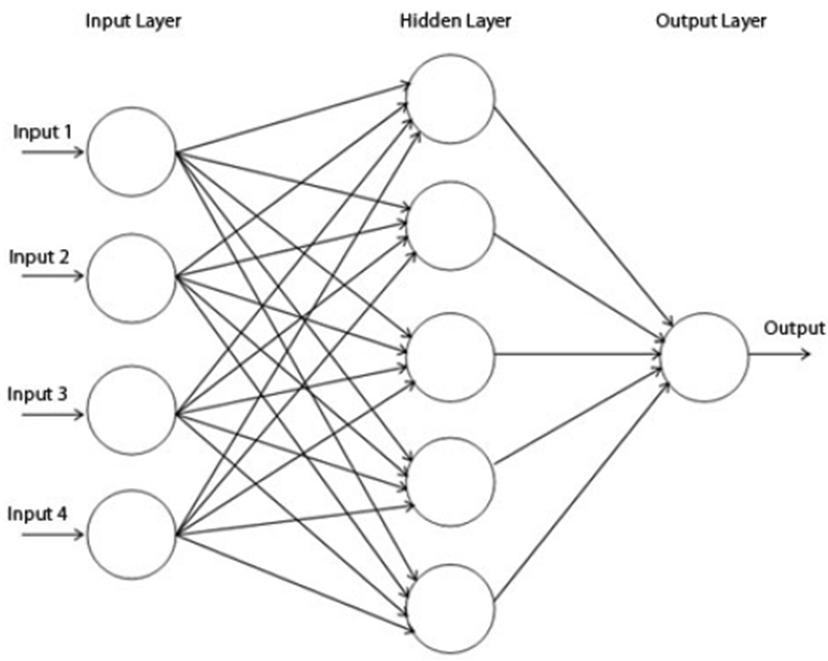
\includegraphics[width=0.5\linewidth]{Pictures/fnn.png}
  \caption{\hl{NEED PICTURE OF MY FNN REAL AMOUNT OF LAYERS Fully connected FeedForward Neural Network with a single hidden layer and one output neuron.}}
  \label{fig:fnn}
\end{figure}
\fi

\iffalse
represented as a chain of a function per layer in the model as e.g. $f(x)=f^{(3)}(f^{(2)}(f^{(1(x)})))$ which is a representation for a model with
two hidden layers as shown in figure \ref{fig:fnn_la}.  Here $f^{(1)}$ and $f^{(2)}$ are the functions of the
first and second hidden layer respectively. The outermost function $f^{(3)}$ is the function for the output layer. We can describe the first layer as $x_i = h_i^{(0)}$, such that the first layer is the 0'th. 
\fi

\subsection{Universal Approximation Theorem}
One of the unique properties of neural networks is that they can compute any function at all and can be approximated by any Borel measurable function [\cite{hornik1991approximation}]. A more straightforward explanation is that the Universal Approximation Theorem states that a Neural Network with one hidden layer can approximate any continuous function for inputs within a finite-dimensional space to another with any desired non-zero amount of error, provided that the Network is given enough hidden units. However, it does not state how large this Network needs to solve the given problem, so this is still done by trial and error methods.



\section{Training of a Neural Network}
feedforward neural networks are mainly used for supervised learning where the data to be learned is not sequential nor time-dependent. This implies that we know the correct output $y$ for each observation $x$. What the system produces is an estimate of $\hat{y}$ (the true y).
The goal of the machine learning approach is to find a weight and bias configuration for each layer that captures the quintessence of the presented data set, that make the estimate of y for each training
observation as close as possible to $\hat{y}$.
Currently, the Network is very much dependent on the training data-set. It should ideally include all kinds of combinations of possible inputs. This can be difficult to do in practice and the available data-sets are therefore typically split randomly into three
categories: \emph{training}, \emph{validation}, and \emph{test} set.\\

The \textbf{training set} is the actual data set that we use to train the model (weights and biases in the case of a Neural Network). The model sees and learns from this data. 
We will need a loss function that models the distance between the system output and the expected output.
The commonly used technique to train the model is by some variation of Gradient Descent \acrshortrshort{GD}. GD algorithms try to minimize a particular loss or cost function with respect to a given weight configuration.
The \textbf{validation set} is used to provide an unbiased evaluation if a model fits on the training data-set. This tells how to change the Network's weights and biases overall behavior, also known as tuning hyperparameters. The evaluation becomes more biased as a skill on the validation data-set is incorporated into the structure of the model. To reduce the risk of overfitting, the optimization
should be stopped as soon as the error on the validation set is not decreasing
any more. 
Generally, over-fitting occurs when a model learns the training data set too well, performing smoothly on the training data set but can not seem to work on a different sample [\cite{Kriesel2007NeuralNetworks}] 
This is one of the other methods applied in machine learning to achieve a generalization over previously unseen data points. Because the information of the validation set is leaking into the Network via the early stopping criterion, a third data set is needed to evaluate the actual performance and generalization of the Network. This third set is called the \textbf{test set}.
The test set is a benchmark used to evaluate the model and is only used once a model is thoroughly trained. However, the focus in this project is to accelerate an already trained model and does therefore not have to be taught any further.


\iffalse
\hl{FNNs contain many good advantages of training data. However, there are also some disadvantages. Backpropagation algorithms, which is this method for calculating the gradient of the error function concerning the Neural Network's weights, typically need vast amounts of data to train the Network. When using gradient descent, the steps have to be small enough not to jump over the desired minima,
which leads to very long training times. Data training can lead to unexplained results if it does not
properly represent the possible parameter space. It will then be more difficult to interpret how the Network came to a specific result, as the weight matrices do not represent traceable reasoning or logic. }
\fi

\begin{figure}
  \centering
  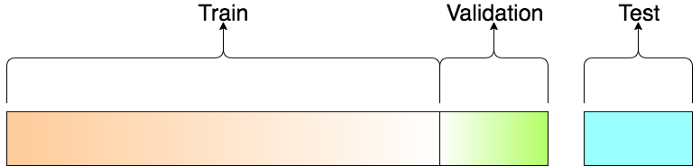
\includegraphics[width=0.5\linewidth]{Pictures/splitdata.png}
  \caption{All data used for training a ML model, split up in a \emph{training}, \emph{validation}, and \emph{test} set}
  \label{fig:fnn}
\end{figure}

\iffalse
\subsubsection{Loss function}

The most commonly used loss function in Neural Networks is the \textbf{cross-entropy loss} when optimizing classification models. We will use this loss function when training our model. It tells us how good our Neural Network is for a specific task.
Cross-entropy loss measures the performance of a classification model whose output is a probability value between 0 and 1. Cross-entropy loss increases as the predicted probability diverge from the actual label, depending on the classification and the activation function used for the output layer.
 The loss function is given by:

\begin{equation}
L(y,\hat{y}) = \frac{}{}
\end{equation}




\section{Gradient descent}
\label{sec:GD}
\fi

\newpage

\section{Our FNN model}
Now that we have the background, we can start looking at the provided model, which is written in Python using the \texttt{Pytorch} library. 
\subsection{Pytorch}

PyTorch is an open-source machine learning library based on the Torch library used for applications such as computer vision and NLP [\cite{pybook}]. It is an open-source library maintained mainly through Facebook’s AI research group.
Unlike other popular frameworks like TensorFlow, which uses static computation graphs, PyTorch uses dynamic computation, allowing greater flexibility in building complex architectures. It uses core Python concepts like classes, structures, and conditional loops, which are easier to understand intuitively. This makes it a lot simpler than other frameworks, such as TensorFlow that incorporates their programming style.
To understand how the model is built, we will quickly go through some features o the PyTorch used in the given script. \\


\subsection{Torch}
PyTorch defines a class called \texttt{Torch.Tensor} which contains data structures for multi-dimensional tensors and mathematical operations. It stores and operates on homogeneous multidimensional rectangular arrays of numbers. "PyTorch Tensors are similar to NumPy Arrays but can also be operated on a CUDA-capable Nvidia GPU.
Additionally, it provides many utilities for efficient serializing of Tensors and arbitrary types, and other valuable utilities" [\cite{py}].



\subsection{Torch.nn}
The \texttt{Torch. nn} PyTorch auto grad makes it easy to define computational graphs and take gradients, but raw auto grad can be a bit too low-level for defining complex Neural Networks. This is where the nn module comes in handy. This model uses \texttt{nn.module} and \texttt{nn.parameter}. The \texttt{nn.module} performs operations on tensors. Modules are implemented as subclasses of the \texttt{torch.nn.module} class. All modules are callable and can be composed together to create complex functions.
the \texttt{nn.parameter} is a tensor that sub-classes the Variable class.
The difference between a variable and a parameter comes in when associated with a module. When a parameter is associated with a module as a model attribute, it automatically gets added to the parameter list and can be accessed using the 'parameters' iterator. \\

The provided FNN model takes in an input $x$ and a target $y$. The weights and data are generated randomly.
I started with a minimal data set to understand each process going through the model to understand all the calculations. This FeedForward Neural Network model consists of two layers shown in Listing \ref{lst:layers}. 
This model is a part of a more extensive pipeline where the models are trained to recognize features that indicate an upcoming increase or decrease in the market pricing and bid accordingly.
Deep Learning methods, while known in general to be highly successful in terms of accuracy, also carry a curse of heavy computations with them. Therefore, we will implement it with SME in the next section and test if we can keep the accuracy and accelerate the inference.


\iffalse
\begin{listing}
  \inputminted{python}{codesnippets/forward.py}
  \caption{Forward function calling all layers used in the FeedForward model}
  \label{lst:forward}
\end{listing}
\fi

\begin{listing}
  \inputminted{python}{codesnippets/fnn.py}
  \caption{The different layers and functions used in the FNN Network}
  \label{lst:layers}
\end{listing}






\chapter{Implementation}
\label{cha:implementation}
\epigraph{
  \hypersetup{linkcolor=bgwhite}

This chapter describes the implementation and gives an overview of the translation of the FNN model to SME. The purpose is to show the structure and thoughts throughout the development of the final SME model. We will highlight the most important technical considerations made during the implementation and how the system was set given the previous chapters' theoretical background. This will be illustrated through explanations and code snippets.
%\hl{When the model is built up in SME, the next step would be to test the model by using simulations in SME. This is done straightforward, given that SME can handle floating points during the simulations. However, it does not work when implementing the model on hardware offered that SME is still taking floating points, so we need to quantize the data. To make this, several approaches had to be done.}



 % Chapter~\ref{cha:anomaly_detection};  
  \hypersetup{linkcolor=linkblue}
}

\iffalse
\section{Thoughts behind the implementation (IS this necessary??)}%
\label{sub:the_journey}

\hl{During the process of working on this thesis, I was not sure how much of the programming and hardware part I was able to learn and implement. However, it was interesting to see how a physicist lacking programming experience, especially with no experience in hardware design, could understand and build a structure of hardware working with high-level code. Therefore, a lot of time and energy was put into the computational parts such as learning - C\texthash, object-orientated programming, machine learning, simulations through SME, understanding time circuits, and generalizing everything such that it can be used for different FNN models and implemented on to an FPGA. My journey to the final code has been a development of exploring different structures and setups of the code, which has been rewritten and updated multiple times.} \\
\fi 

\section{The architecture of SME\_ML}%
\label{sec:SME_ML}
Having the theoretical background behind FNN and SME, we will in this section introduce the implementation of the FNN model in SME and describe some of the essential parts.
The code that was developed in this work \textbf{ML\_SME\_FPGA} can be found on Github [\cite{Github}]. The result is generalized such that each function can be used for different purposes on an FPGA.  
The ultimate goal is to find methods for transpiling that
can be generalized to different FNN problems.
The python code provided by the HFT company who wants to remain anonymous was made in python with the \emph{Pytorch} library, which I after that translated to C\#, using almost no built-in libraries. This was because we wanted to understand the data structure of all operations such that it would be easier to implement with SME.
The main intention of each language is different, and therefore the transpiling of a process in the given Python code to an SME process might not be completely trivial. However, the automatic parallelization of the network is still helpful for users wanting to run the model on an FPGA.
\\

Before getting into the concrete implementation detailing the model, let us restate the purpose of the FNN model and how we want to go from a Python model to full implementation on an FPGA.
Based on an input sequence $\mathbf{x}$ and a set of trained weights $\mathbf{w_i}$, a model is made to predict a $\mathbf{y}$ in Pytorch, which we will recreate in SME. We will do this by being aware of timing and restricted clock cycles such that the calculations run correctly and independently of each other. The final model works in the following way:

\begin{enumerate}
    \item \textbf{Takes in} the input sequence $\mathbf{x}$ and the weights $\mathbf{w_i}$. 
    \item \textbf{Runs} the FNN model
    \item \textbf{Compares} the SME- with the Pytorch -output
\end{enumerate}
The whole architecture is divided into several sections, but to execute this, you need to load your data in the \texttt{Deflib/data} file and run the \texttt{FNN} folder. The \texttt{FNN} calls in all the other modules, which can be found in \textbf{ML\_SME\_FPGA}. In the following sections, we will describe some specific implementation details worth noting. \\

\newpage

\section{Matrix multiplication in SME}
Each module is designed as an individual simulation setup to be tested separately from the rest of the system. A further explanation about how to test the modules can be found in Section~\ref{sec:simulation}.
To give an idea of how each function is structured in the core of the FNN, we will look at a concrete example; the \ttt{Matmul} function. 
To understand the development of the process, we will go through the steps of going from the python to SME model. This consists of the following main steps:

\begin{itemize}
    \item Translation from python to C\#
    \item Write in the SME framework
    \item Re-structure functions to run independently
\end{itemize}

\subsection{FNN in C\#}
For this example, we will only focus on this specific line from the given FNN model shown again in listing ~\ref{lst:mm}. This function calculates the matrix multiplication in the first layer of the model.
As we can see in listing \ref{lst:mm}, before the matrix multiplication, there is a need for a reshaping and transposing of the function, but we will only focus on the matrix multiplication for now. 
I had to write the function out in C\#.
This is generally not necessary to do first, but beneficial since it is needed for the testing. Another reason and something to be aware of is that this is done because in SME in specific situations, calling C\# libraries will not translate directly to VHDL, which is the goal. This happens when using the \texttt{SimpleProcess}. The global hidden clock drives this process with the OnTrigger function that is triggered once in each clock cycle [\cite{LennartJones}].
The \texttt{Matmul} function is shown in Listing~\ref{lst:mm_func}. Translating all lines to the necessary functions such as reshape, transpose, sigmoid, etc. It was done and tested with several examples to ensure it worked for different cases. I manually tested all functions to start with. This was my way to incorporate learning C\# programming. \\

The next step was recreating the FNN model in C\#, so it looked close to the python script. 
A snippet of the model from C\# is shown Listing~\ref{lst:mm_cs}.
Specific data was generated and tested a reasonable amount of times on both models to ensure that they both gave the same output. %This part could probably have been avoided if I had sufficient knowledge about machine learning and programming, but it was done for me to understand each step of the process and the structure of the code. Also, this made the SME part a notch easier to write.

\begin{listing}
  \inputminted{python}{codesnippets/mm.py}
  \caption{Matrix multiplication in python using the \texttt{Pytorch} library among other operations }
  \label{lst:mm}
\end{listing}

\begin{listing}
  \inputminted{csharp}{codesnippets/mm_func.cs}
  \caption{Matrix multiplication written out in C\# }
  \label{lst:mm_func}
\end{listing}


\iffalse
\begin{figure}[]
 \begin{minipage}{0.5\textwidth}
  \centering
   \inputminted{python}{codesnippets/mm.py}
  \captionof{listing}{Sub caption}
 \end{minipage}
 \begin{minipage}{0.6\textwidth}
  \centering
    \inputminted{csharp}{codesnippets/mm.cs}
  \captionof{listing}{Another sub caption}
 \end{minipage}
 \captionof{listing}{SomeCaption}
  \label{lst:representation_examples}
\end{figure}
\fi


\begin{listing}
  \inputminted{csharp}{codesnippets/mm.cs}
  \caption{The C\# version of listing \ref{lst:mm_func}}
  \label{lst:mm_cs}
\end{listing}

\section{Write to SME}
%This was the most challenging part of the work since the mindset behind hardware architecture was very new for me. 
The Sigmoid function was made to get introduced to the SME framework, which is shown in \ref{appendix:Sme_guide}. There are many ways to build a function in SME, and this was also the case for the \texttt{Matmul} process. Several block diagrams were made. The final block diagram is shown in Figure~\ref{fig:mm_block_old} containing the methods and busses that were necessary for the function to take in data, calculate correctly in the correct order and give an output. Because matrix multiplication is a combination of multiplication and addition, where the operations are dependent on each other, we need other functions to hold on to data and forward them. This is where the different processes come in. \\
The following sections will explain the different processes from the pipeline used in the implementation.


\begin{figure}
  \centering
  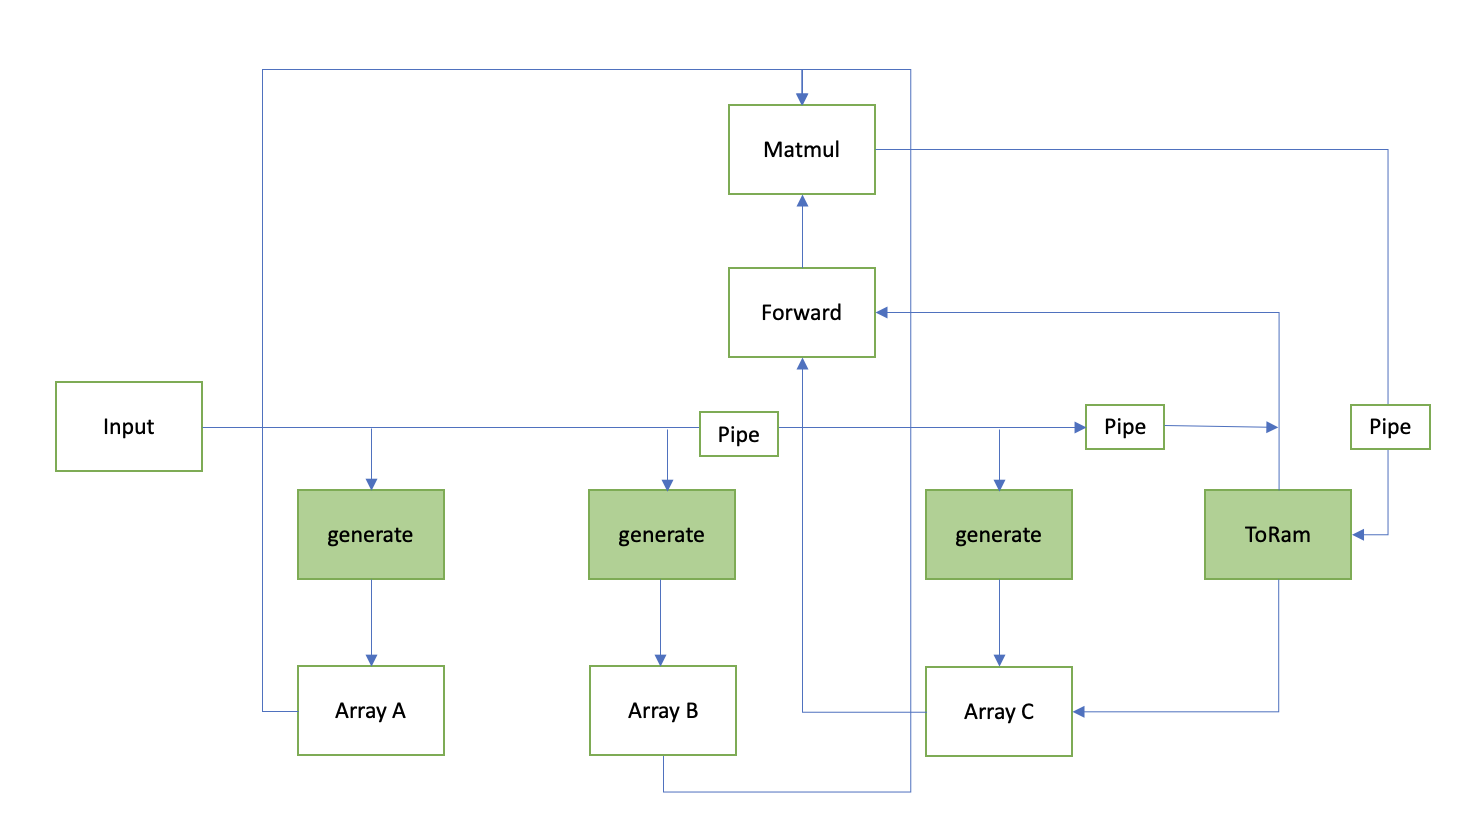
\includegraphics[width=1\linewidth]{Pictures/mm_block_old.png}
  \caption{Block diagram of the \texttt{Matmul} module. The colored boxes represent the non-clocked processes, since they just are empty 'boxes' with the only purpose of changing the bus type going through them.}
  \label{fig:mm_block_old}
\end{figure}

\subsection{Generate}
The generate function takes the data in their given sizes and outputs as a flat array since the $Ram$ only takes flat data. The actual shapes will be defined when addressing the data, i.e., in \texttt{MatmulIndex}. 
This process has an input bus that holds the base address, and the output bus reads the data.

\subsubsection{Implementation}
To implement the unit, we create an SME process. 
In SME, a process cannot make matrices from lists, as lists are dynamically allocated. However, we can make them as arrays as these can be statically allocated. It needs to be clocked, meaning the unit will activate on a rising clock edge, as it will be part of a closed-loop circuit when we later connect the units. If no unit is clocked in a closed-loop, there is no way of knowing where to begin sending signals, and if translated to hardware, one would get a short circuit, which would destroy the chip.
Because the process is clocked, when it reads the following address input, it will contain the address calculated in the previous clock cycle, as the bus has not been updated yet. This would then be the correct address in the current clock cycle.
This is because the bus has not been updated yet. This would then be the correct address in the current clock cycle. 

\begin{listing}
  \inputminted{csharp}{codesnippets/generate.cs}
  \caption{The generate process}
  \label{lst:datagenerator}
\end{listing}

\subsection{Matmul and Matmulindex}

\subsubsection{Matmul}
The \texttt{Matmul} is implemented as a pipeline, where each sub computation is performed in a single clock cycle.
The \texttt{Matmul} process takes in the Block RAM that holds the matrices, A and B used for the computation $C += A * B$. When C is calculated, it gets sent through the \texttt{Forward} process and will continue into the \texttt{Matmul}. When the calculation is ready, it will add C to the next A and B in the matrix. These ports are named Array\_A, Array\_B, and Array\_C, respectively, which are all input busses, meaning the data are stored in these arrays.

\subsubsection{Implementation}
This process takes four busses and outputs the calculated value.
Three input busses are the matrices Array\_A, Array\_B, and Array\_C.
It also consists of one input-bus, \emph{input\_pipe}, which is a base holding the base address. 
To give an idea of how a process looks like, we will show the whole \texttt{SimpleProcess} once, including how we define the busses and the structure of the process. The actual relevant part here is from line 28, where we define an \texttt{OnTick}. This is the part that runs over one clock cycle. If the following input is ready, we will calculate the matrix multiplication. With this, we can check if it takes data in. From now on, I will only show the \texttt{OnTick} functions since they are more relevant.
Additionally, since all data needs to be handled as flat lists for the matrices, we must define another process that keeps track of the real matrix shapes. This function is called \texttt{MatmulIndex}. 

\iffalse
\begin{listing}
  \inputminted{csharp}{codesnippets/Matmul_old.cs}
  \caption{The whole process for the \texttt{Matmul} calculations including the structure with busses used}
\end{listing}
\fi

\subsubsection{MatmulIndex}
\ttt{MatmulIndex} keeps track of the indices in the matrices. It can be thought of as a register that holds the current instruction's address. This is very important to keep track of where we are in the matrix. It is also here the dimensions of the matrices are being taken into account.
The input busses contains of \emph{controlA} and \emph{controlB}. The two control busses both contain a \texttt{bool} value which checks whether the dimensions of the input data are correct.
The output busses take the addresses from all the matrices, A, B, and C.
The last \emph{controlout} bus specifies the sizes and validity of the respective matrices.

\subsubsection{Implementation}

All the control busses are made from the \ttt{IndexControl} bus, which consists of the following fields: a boolean indicating whether the data is valid, a string holding the base address, an int indicating the access stride, and an int specifying the size of the matrix.
The main restriction with the \ttt{Matmul} function is the multiplication being dependent on the accumulation, which is performed within a single clock cycle. To make sure we hold the right data at the correct time, we add a process to the pipeline called \texttt{Forward}.


\begin{listing}
  \inputminted{csharp}{codesnippets/matmulind.cs}
  \caption{The Matmulindex }
  \label{lst:datagenerator}
\end{listing}



\iffalse
\begin{enumerate}
    \item \textbf{generate}
    \item \textbf{Matmulindex}, adressing the index in the matrices
    \item \textbf{pipe}
    \item \textbf{forward}
    \item \textbf{Matmul}
    \item \textbf{ToRam}
    
\end{enumerate}
\fi

\begin{figure}
    \centering
    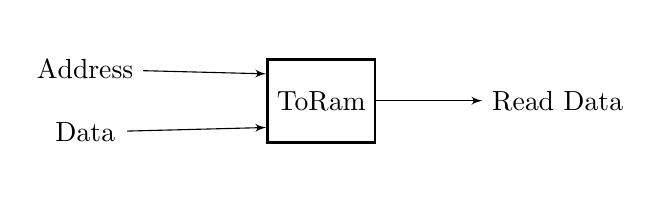
\begin{tikzpicture}
        \node[block] (mem) at (0,0) {ToRam};
        \node[empty] (addr) at (-3,0.4) {Address};
        \node[empty] (data) at (-3,-0.4) {Data};

       
        \node[empty] (readdata) at (3, 0) {Read Data};

        \path[draw, ->] (addr) -- (mem.154);
        \path[draw, ->] (data) -- (mem.206);
        \path[draw, ->] (mem) -- (readdata);
    \end{tikzpicture}
    \caption{The ToRam Unit.}
    \label{fig:mem}
\end{figure}


\subsection{ToRam}
The ToRam Unit is like Generate, but for the write port to the memory. This is where the final calculations are stored. The FPGA can either read or write to the Memory
Unit in a single cycle. The Unit has two inputs: \ttt{v\_input} (the data) and \ttt{index} (the address).
It has a single output: \texttt{output}, where it writes the data. The ToRam Unit and its connections can be
seen in Figure~\ref{fig:mem}.

\subsubsection*{Implementation}
The ToRam process takes the Address and Data and should all contain a \texttt{int} value. 
The memory part should be an array, and
should read and write 
On each clock tick, the process should check if the \texttt{Index} flag is
set, in which case it should read the value on the Address bus and output the
the value stored in memory at the read address. 





 \subsection{Pipe}
Since parts of the Matmul function are dependent on its previous calculation,
there will be issues withholding the same positions in the indexing when running over each clock cycle. It is possible to write an indexing process in a way that reads and writes simultaneously; nevertheless, this will take a longer time when running the code. This is not very efficient, as the longest path in the processor determines the processor’s clock rate. A path
in a design is the components that a signal goes through until it reaches a
'ready' state. A ready state in an FPGA tells that the signals are safely
stored in the registers. A longer path implies a lower clock rate.
So to increase the clock rate, there is a need to decrease the longest path in the processor. For this, we introduce \ttt{Pipes}.\\
Pipes are registers in the processor, where all the values computed so far are
temporarily stored. It takes all of its inputs and holds them until the next
clock tick, where it will forward the values it is holding. This ensures that the data does not have to travel as far until it has reached a ready state.

\subsubsection*{Implementation}
Implementing the Pipe Unit should be done with an SME process. 
To implement the pipe function, we write the same function for the $genereate$ function.
On each clock tick, the process should check if the \texttt{Ready} flag is
set, in which case it should read the value on the Address bus and output the
the value stored in memory at the read address.


\subsection{Forwarding}
Since the Matmul calculation output depends on the previous output, we need to store the different outputs and require a process that can compare the other addresses and results and forward the final output.
The Forwarding Unit looks at the address $new\_input$ and check if the calculated value corresponds with the previous calculated address $old\_input$. If they fit, it will forward the calculated value 
from the \emph{Matmulindex} function to 
the Matmul stage. The structure of the simplified processor with the forwarding unit can be seen in Listing~\ref{lst:forward}.

\subsubsection*{Implementation}
Implementing the Forwarding Unit should be done with an SME process. As it
Interact with the Matmul stage should be put in the Matmul stage.
The unit consists of five busses.
The first four busses are input busses which we take in. They consist of two busses: the pipes that hold the $old\_input$ and $new\_input$ addresses. The following two busses are the calculated values of the old and new output, and the last bus is an output bus that forwards the value.


\begin{listing}
  \inputminted{csharp}{codesnippets/forward.cs}
  \caption{Forward process}
  \label{lst:forward}
\end{listing}


\section{The FNN model in SME}
For the rest of the needed functions in the network, the main challenge has been making sure that the right data and indices are correct.
However, they were built on the same principles, where the main difference in all of them was the structure of the processes sending the indices
around depending on size and dimension. 
The processes around the main functions in the FNN models, which are used more than once, are saved in the module \textbf{Deflib}. This is also where the data, simulation, and C\# version of the FNN models are kept. The rest of the relevant processes needed have their module.

When I first tested all the functions, they all depended on each other, leaving the debugging process very long and hard. Therefore there was a need to pipeline them all so that they could be modified and tested independently. 
All modules in the FNN simulation have been designed to be pipelined. This was an important design consideration because each module consisted of many individual calculations. If the system had to wait for each calculation to finish, it would increase the runtime considerably.
Each module setup consists of one or more \texttt{SimpleProcesses} and at least one \texttt{SimulationProcess} which generates input data for the network.
The pipelined structure results in each clock cycle, all sections of the modules are in use. The pipelined system also means that we cannot calculate something in one clock cycle and expect it still to be a couple of clock cycles down the line. This means that if a result from a calculation needs to be used later on, we either have to save it into the RAM or send it through the pipeline until it is required. With data always needed at a specific point in time, it makes sense to send it through the pipeline.
Understanding how a module can be built and connected leads us to the rest of the modules and their purpose in the FNN\_SME model. The raw connection between them is illustrated in fig.~\ref{fig:fnn_sme}. A lot of work was put into each module, making sure that it forwarded the correct data and sizes and ensuring that the calculations were executed at the correct time. The fully connected \acrshort{FNN} model can be seen in Figure~\ref{fig:fnn_block_sme}. The instructions on the addresses need to be given explicitly, such that everything gets sent around in the right order.
This means that no matter how much we try to generalize the modules, the addresses need to be changed if desired with the model. \\

Each module consists of a process, program, and simulation file. In the process file, there are two different processes. The first is the indexing of the input. Important notice when working with SME is that the dimensions are fixed to an extend. The biggest problem is that the RAM cannot change after the hardware has been generated. Processes such as index calculation are done dynamically and could easily be changed during run-time since they receive all of the dimensions on the control buses. If one were to truly fix all of the sizes, additional optimizations could be introduced since we don't have to have the complete precision given by a 32-bit number when there is only a need to count to 16.



\subsubsection{Transpose}
The transpose module is the only function not containing a natural process function since the function in itself changes the address of indices by transposing them.
To give a general idea of how the indexing process looks for most of the modules, an example of the \texttt{TransposeIndex} process is shown in Listing~\ref{lst:transpose}. The most relevant part in the indices getting addressed from lines 1-18. The rest are statements forwarding the information if the indexing holds. 

\begin{listing}
  \inputminted{csharp}{codesnippets/transpose.cs}
  \caption{Transpose index, addressing a }
  \label{lst:transpose}
\end{listing}



\begin{figure}
  \centering
  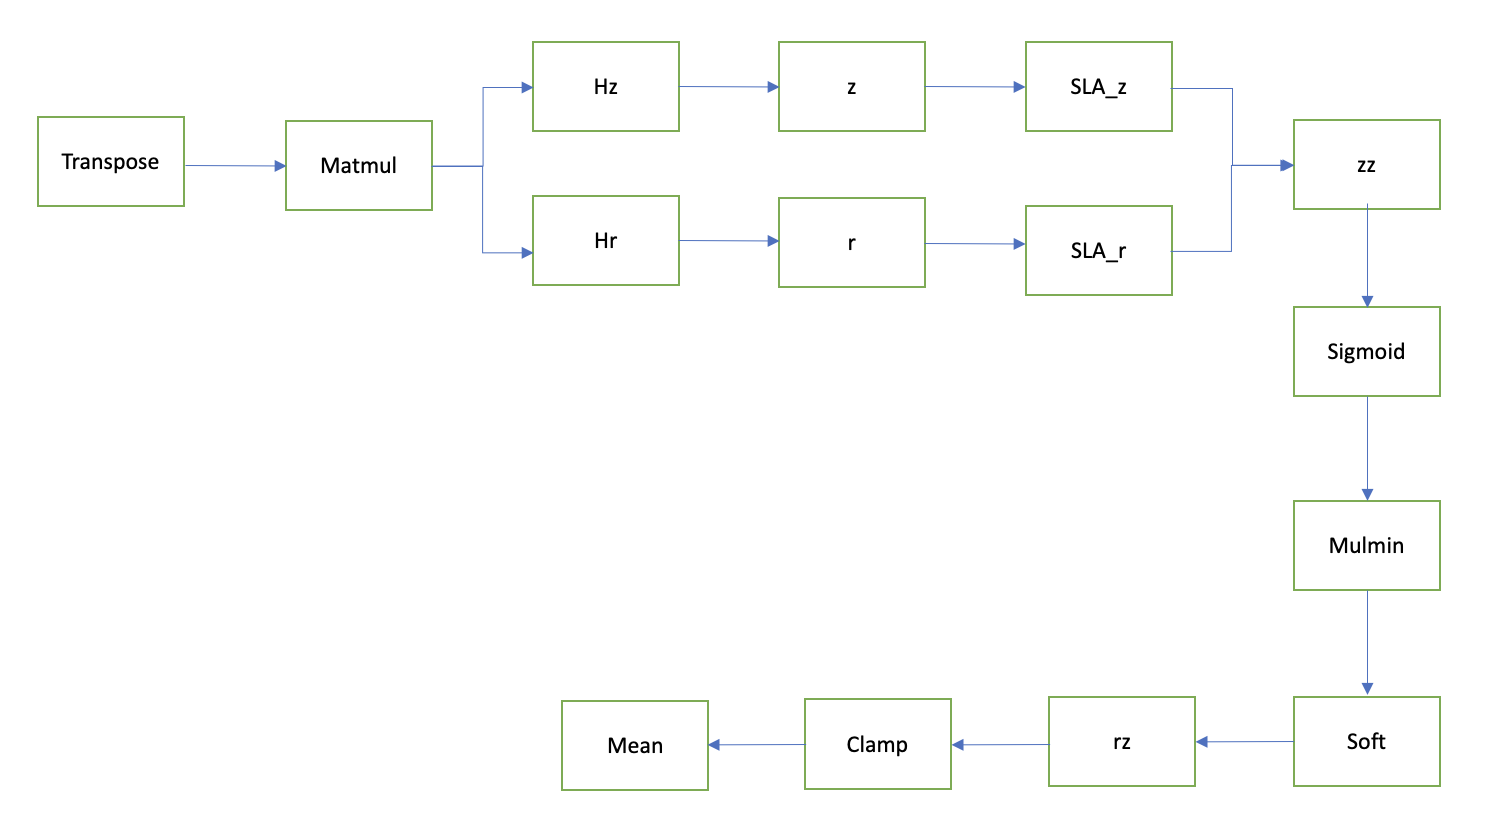
\includegraphics[width=1\linewidth]{Pictures/fnn_sme.png}
  \caption{
  }
  \label{fig:fnn_sme}
\end{figure}

\begin{figure}
  \centering
  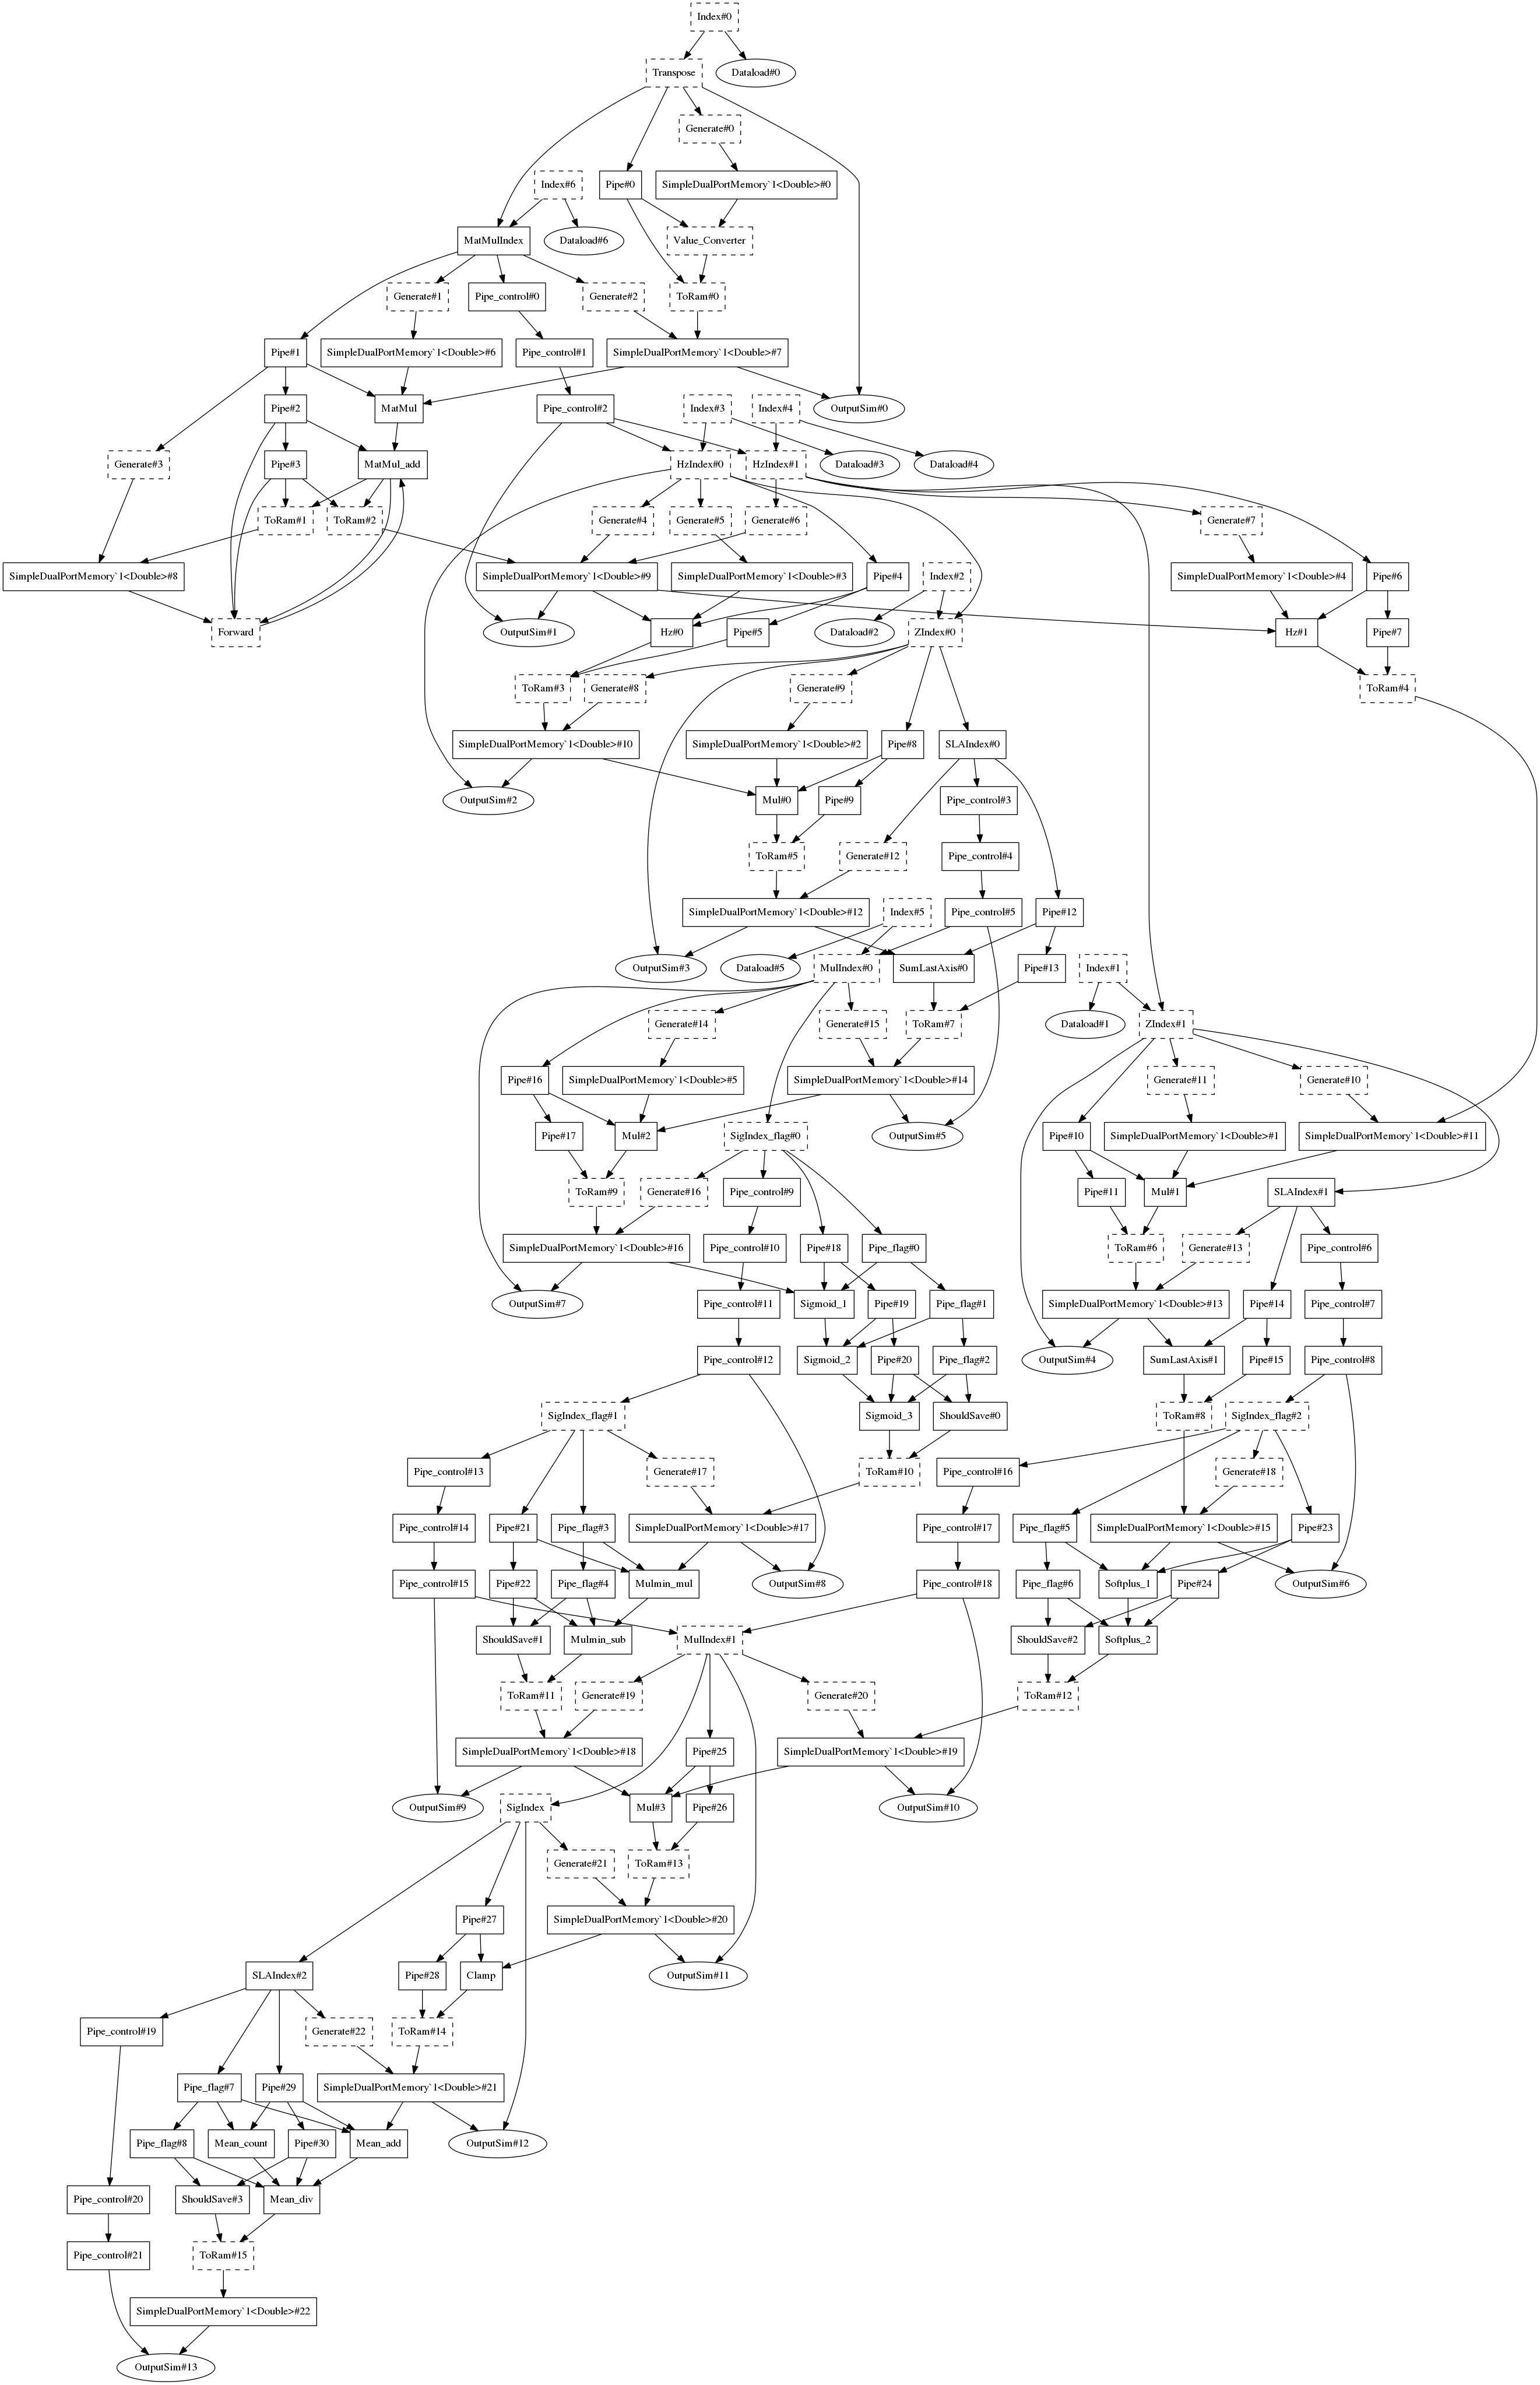
\includegraphics[width=1\linewidth]{Pictures/feedforward_diagram.png}
  \caption{Block diagram of the whole module  This diagram is not including all the busses used, but shows the connection of all the processes used}
  \label{fig:fnn_block_sme}
\end{figure}

\section{Quantization of Neural Networks}
\label{sub:quantization}
We are interested in comparing the results from the Pytorch model with the SME model, making sure that the functions are written correctly. However, the given data from the company is using floating points for their data. At the same time, the SME framework supports floats when simulating but does not yet have floating points implemented for deploying on an FPGA. One solution to compare the Pytorch and SME models would be to quantize the data in Python. \emph{Pytorch} has made it possible to quantize data while training the model. Quantization is a technique that stores tensors at lower bit widths than floating-point precision. A quantized model performs some or all of the operations on tensors with integers rather than floating-point values. This allows for a more compact model representation and the use of high-performance vectorized operations on many hardware platforms [\cite{quantization_pytorch}]. Quantization is primarily a technique to speed up inference, and only the forward pass is supported for quantized operators.
So to evaluate the data, we would need to train the models for quantization. Our focus is not really about training the model most efficiently but instead using it as a tool to get integers out.
The \emph{Pytorch} library arguments that it supports integer 8bit (INT8) quantization compared to typical floating-point 32bit models allowing for a 4x reduction in the model size and a 4x reduction in memory bandwidth requirements [\cite{quantization_pytorch}]. There are different approaches to quantizing the model depending on the whole pipeline structure: post-training dynamic quantization, post-training static quantization, and aware quantization training. Since this is just a tiny part of a more prominent structure, the simplest version would be enough to see if it works. \\

I chose to play with the python model to start with since this library seemed straightforward, but I must have missed something while working with it.
The instructions stated that applying the quantization on the model and training them would be needed to get a set of weighted integers. However, after several tries, the model wouldn't seem to save it any differently. I used the time to train the model and used all the different quantization approaches without any luck. Since this took too long to figure out and time was getting short, I decided to look into another way of getting the SME model to work with floating points. 


\section{ONNX}

An interesting thought that came up during this implementation was the question about saving \emph{Pytorch} models and uploading them directly in C\#, without translating manually and thereby saving a lot of time. 
With the PyTorch framework, it is possible to train a model, save it and download it as an ONNX file to run locally with Windows machine learning in C\#. This would save time for future work going from one framework to another and rewrite the C\# code into SME. 
We could also test other models containing the same operations we have implemented in SME and compare how fast they execute compared to each other.
This is where ONNX comes in handy. ONNX is an open format built to represent machine learning models. ONNX defines a standard set of the building blocks of machine learning and deep learning models. It generates a common file format to enable machine learning developers to use models with various frameworks, tools, run-times, and compilers.
We managed to save and download the model but could not open a translated \texttt{Pytorch} version in C\#. However, several attempts to use ONNX to convert different deep learning models were made without success. 

\newpage


\section{SME and floating points}
Since the time was running out, I decided to save this idea of optimizing the performance and focus on getting this piece of code working. 
Unlike with CPUs/GPUs, FPGAs are more limited in the available calculation methods, i.e., the SimpleProcess [\cite{LennartJones}]. We can not just import a math library to do advanced functions. Specific calculations have a drastically better performance than, e.g., division, and choosing wrong will reduce the performance of the system [\cite{LennartJones}]. Since we are targeting Xilinx boards, we are restricted to the \ac{IP} blocks that they provide for floating-point numbers. To be able to do calculations consisting of more than one operation in the \texttt{SimpleProcess} for the different modules used in the FNN model, we had to do some restructuring to fit it into the possible IP blocks provided by Xilinx. This means we will have to split the processes up into doing only one calculation, then several calculations in one process.\\

As an example, we will look at the \texttt{Matmul} function again. The original version of this process which calculates the \texttt{Matmul} consists of different operations such as accumulation and multiplications happening at the same time in the same process. However, if this should work for floating points, we will need to split it up so that the FPGA can more easily connect all operations.
This is therefor done by splitting the \texttt{Matmul} Process in two processes; \texttt{Matmul\_Add} and \texttt{Matmul\_Mul}.
On each clock cycle, one value is read from the A and B matrix, streamed to the Multiplier. The Accumulator keeps adding its input until the address for matrix C changes, writing the value to C. 
To ensure that all data gets sent at the proper clock cycle, some flags are set every time a result needs to be saved. We also need more pipes to hold the data until it is sent to the following process. The new structure of the matrix multiplication is shown as a block diagram in fig~\ref{fig:mm_diagram}. 


%På FPGA er floating-point enhederne lidt særlige, så for at det bliver effektivt skal værktøjet kunne gætte hvilke operationer der passer til hvilken hardware komponent. Ved at dele dem op til separate processer bliver det muligt for værktøjet at mappe dem korrekt.


\begin{figure}
  \centering
  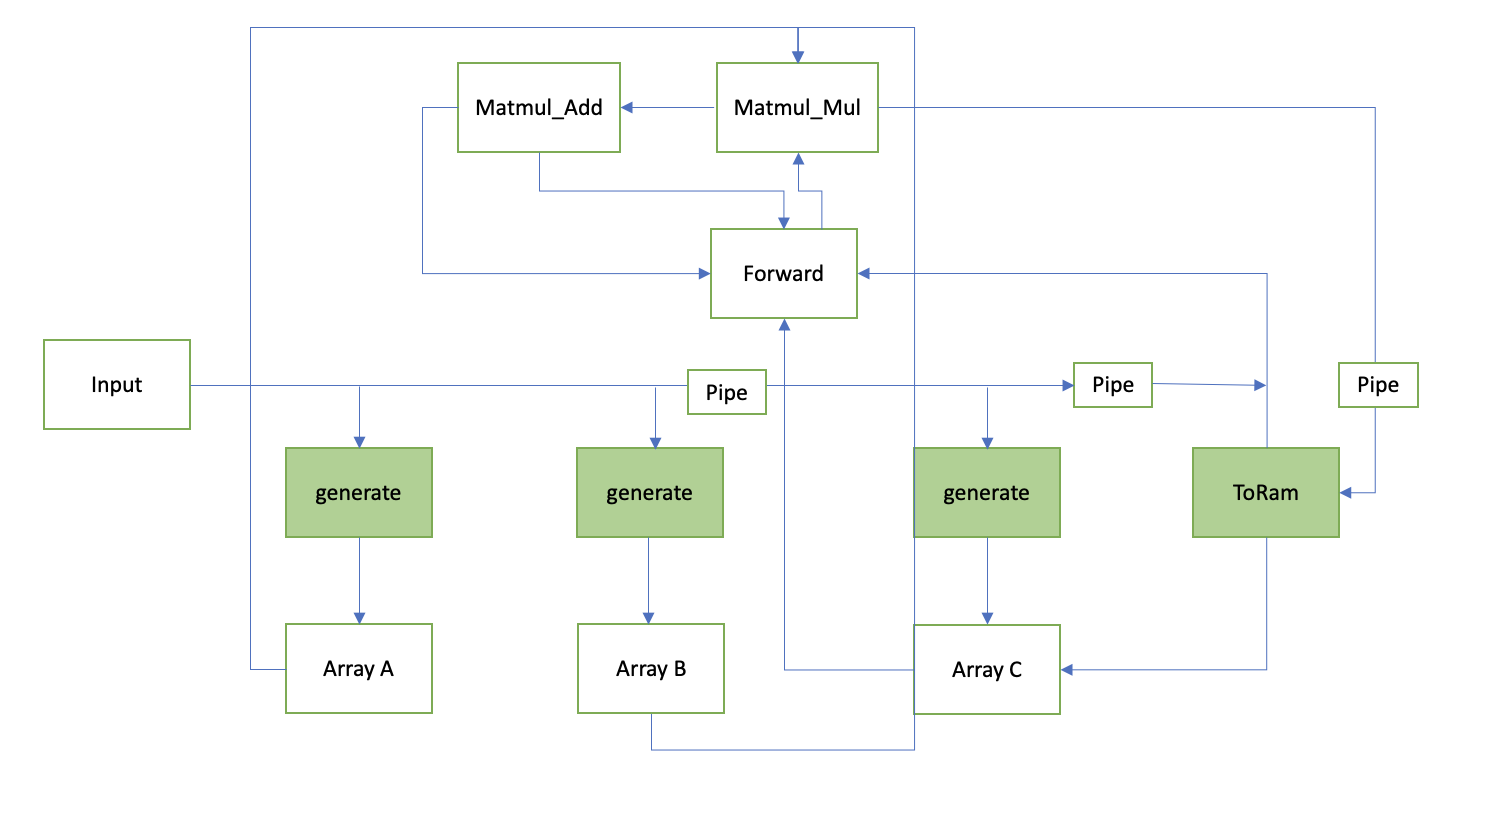
\includegraphics[width=0.8\linewidth]{Pictures/mm_blocks.png}
  \caption{Block diagram of the restructured \texttt{Matmul} module. The \texttt{Matmul} process is splitted up to \texttt{Matmul\_Add} and \texttt{Matmul\_Mul}}
  \label{fig:mm_diagram}
\end{figure}

\iffalse
\begin{listing}
  \inputminted{csharp}{codesnippets/mean_before.cs}
  \caption{Code snippet from the process calculating the mean before splitting up}
  \label{lst:mean_before}
\end{listing}


\begin{listing}
  \inputminted{csharp}{codesnippets/mean_after.cs}
  \caption{Codesnippet from the mean process calculation the mean}
  \label{lst:mean_after}
\end{listing}
\fi


\section{Simulation process}
\label{sec:simulation}

Now, having the structure of the SME feed-forward neural network model, we need to test whether or not it gives the same results as the \texttt{Pytorch} model.
There is a simulation part for each process to test the functions and follow the results. Notably, the final structure results from an iterative process, where the form of testing changed multiple times while building it.
The first simulation to test the functions was built to encompass all the other processes because nothing was pipe-lined and would therefore cause frequent errors. However, we managed to pipeline the structure, such that each module is designed as an individual simulation setup so that it can be tested separately from the whole system. When the modules are connected to the entire FNN network system, one \texttt{SimulationProcess} generates data and verifies the result.
Besides generating input data, the \texttt{SimulationProcess} uses self-made C\# libraries to calculate the results of the simulation as verification for the SME results. \\

Each module is a folder containing a \textbf{process.cs}, \textbf{program.cs} and \textbf{simulation.cs} file. The simulations file generates the expected output, and the test verification happens in \textbf{program.cs}. For instance, when calculating the \texttt{Sigmoid} function, the Testing Simulator will create input data generated from the calculation before, which is from the \texttt{zz} then. While the \texttt{Sigmoid} is calculated, the Testing Simulator will calculate the actual sigmoid function using standard C\#. This way, when \texttt{Sigmoid} gets computed, it is simple to check whether or not these results are as expected. The output will be a bool of true or false depending on if the results match. Often during development, we ran into errors where the calculations were correct, but the timing was wrong, which meant that the signals arrived unaligned, causing the results to be out of sync. By having a standard C\# calculation based on the current input data, it was easy to see how the timing of data communication was misaligned.

The Simulation is constructed using the following steps: A process that takes in the data converts the size and dimensions since the Ram only takes flattened data and simulates each function and compares it to the actual answer from the model.
With this in place, we can test each function and connect them. We are ultimately building the final FNN and testing it concurrently.

\subsection{LoadStage}
The \ttt{LoadStage} is a function that loads the data in, flattens it, and indexes it to the correct size and dimensions. It controls whether the index holds its proper size.
The \ttt{LoadStage} is shown in Listing~\ref{lst:loaddata} and consists of three other other processes:
\begin{itemize}
    \item DataLoad
    \item TestIndexSim
    \item Index
\end{itemize}

The \textbf{DataLoad }reads the CSV file, the total size of the data, and the value of the index. The output is a flat array ready to connect to a given address.
Since all the data comes in a flat array, we need to create a process that has the right dimensions to ensure that the sizes hold up. This is where \textbf{TestIndexSim} comes in. 
In \textbf{TestIndexSim} we overload with up to three dimensions including an index-control. The index control makes sure to output an error if the sizes do not hold up.
When we run the simulations, the sizes get transferred to the other processes with their given measures, which can then handle their actual dimensions.
The \textbf{index} keeps track of where in the program we are located. It can be thought of as a single register, which holds the address of the current instruction.
Further, the indexing process holds the instruction address. The input bus contains the address of the next instruction and the output bus with the current address.

\begin{listing}
  \inputminted{csharp}{codesnippets/loaddata.cs}
  \caption{LoadData process that loads the input and address the data with their correct sizes}
  \label{lst:loaddata}
\end{listing}

\subsection{simulation.cs}
When the data is loaded in with their correct sizes and dimensions, the next step would be to run them through the simulation processes.
Taking the structure of the \ttt{Matmul} Function as the starting point, there needs to be a simulation function to test out the results.
Before performing matrix multiplication, the model reshapes and transposes the data. The simulation process takes in the model, rewritten in C\#, and calculates the predicted outcome. In the \textbf{program.cs} file there are two parts:
The first part takes in all the SME processes written for that specific module and pipelines them to get the whole SME \ttt{Matmul} function; this part is called the \texttt{MatmulStage}. The other half of the \textbf{program.cs} takes in the data, the FNN network from both the C\# version and the SME and compares them inside the \ttt{OutputSim} process. 
The \textbf{OutputSim} is the process that compares the calculated output from SME with the expected output calculated using C\# functions.
To give a more straightforward visualization of the program file, a snippet of code is seen in Listing~\ref{lst:mm_program}.
Here, it calculates the expected Matmul output, generates the SME data, calculates the SME Matmul output, and compares those two at the end with \ttt{OutputSim.cs} which prints a \textbf{True} if the results match.\\


\begin{listing}
  \inputminted{csharp}{codesnippets/matmul_program.cs}
  \caption{Small snippet of code of the \texttt{program.cs} file calculating the matrix multiplication output for the expected and actual output}
  \label{lst:mm_program}
\end{listing} 




\label{sub:quantization}
%The given data from the company uses floating points on their data. The SME framework and does not yet have floating points Incorporated. This is why we need to quantize the data. \emph{Pytorch} has made it possible to do through the training of a model. Even though we evaluate the FNN model in SME, we will only train it in the python code for quantization. Our focus is not the training of the model but to quantizes the data and see if this also will help speed up the process of processing data. Since it is supposed to run faster for integers.\\
%Quantization refers to techniques for performing computations and storing tensors at lower bit widths than floating-point precision. A quantized model executes some or all of the operations on tensors with integers rather than floating-point values. This allows for a more compact model representation and the use of high-performance vectorized operations on many hardware platforms. PyTorch supports integer 8bit (INT8) quantization compared to typical floating-point 32bit (FP32)  models allowing for a 4x reduction in the model size and a 4x reduction in memory bandwidth requirements [\cite{quantization_pytorch}]. Quantization is primarily a technique to speed up inference, and only the forward pass is supported for quantized operators.

\chapter{Results}
\label{cha:results}
\epigraph{
  \hypersetup{linkcolor=bgwhite}


The thesis results will be presented in this chapter, touching upon two key areas. 
%First, the \texttt{simulation} process and data testing will be explained to give an understanding of how to test the model. Second, 
The proposed methodology from the previous chapters will be adopted and tested on the data of the focal company. Conducting this experiment will provide further insight into the speed and performance of the FPGA and how it performs in a real-life setting. 
 

 
  \hypersetup{linkcolor=linkblue}
}






\section{Results}

\begin{table}
\centering
\begin{tabular}{||c|c |c| c| c| c |c||} 
 \hline
 \textbf{Id} & \textbf{Data} & \textbf{input size} & \textbf{hid size} & \textbf{\# networks} & \textbf{max predict} & \textbf{Batch size}\\ [0.5ex] 
 \hline\hline
1 & Test size & 4 & 7 & 5 & 1 & 1 \\ 
2 & Actual sizes & 256 & 96 & 16 & 1 & 1 \\ [1ex] 
 \hline
\end{tabular}
\caption{\textit{Parameters with different sizes used to test the FNN model in SME}}
\label{table:data_size}
\end{table}

\begin{table}
\centering
\begin{tabular}{||c c c c c c||} 
 \hline
Name & Clock rate [MHz] & Logic & Registers & Block RAM  & DSP \\ [0.5ex] 
 \hline\hline
clamp & 191.4975 & 197 & 419 & 0 & 0\\
hzhr & 74.6436 & 711 & 1089 & 1.5 & 10\\
load\_data & 596.3000 & 993 & 2367 & 9.5 & 56\\
matmul & 51.2242 & 596 & 1292 & 9.5 & 9\\
mean & 17.7135 & 1162 & 1372 & 0 & 3\\
mulmin & 51.6022 & 417 & 1037 & 0 & 4\\
rz & 90.6536 & 273 & 526 & 0 & 4\\
sigmoid & 17.7135 & 1933 & 1267 & 0 & 3\\
softplus & 31.1536 & 1188 & 1037 & 0 & 3\\
sumlast & 45.7603 & 846 & 2317 & 1 & 6\\
transpose & 884.9557 & 249 & 403 & 16 & 2\\
z\_r & 77.9301 & 545 & 1041 & 3 & 10\\
zz & 90.6536 & 273 & 526 & 0 & 4\\
FeedForward & 17.7135 & 9121 & 8468 & 20.5 & 110\\
 \hline
\end{tabular}
\caption{
\textit{Small parameter set}. Timing and utilization post Synthesis as reported by Vivado targeting a ZedBoard.}
\label{table:utilization_small}
\end{table}



\begin{table}
\centering
\begin{tabular}{||c c c c c c c||} 
 \hline
name & Clock rate (MHz) & Logic & Registers & LutRAM &  Block RAM & DSP  \\ [0.5ex] 
 \hline\hline
clamp & 184.6722 & 215 & 418 & 48 & 0 & 0\\
hzhr & 74.0686 & 657 & 1117 & 48 & 6 & 10\\
load\_data & 47.6077 & 4198 & 2458 & 2360 & 384 & 56\\
matmul & 51.2243 & 3673 & 1991 & 2288 & 384 & 11\\
mean & 17.7135 & 1162 & 1372 & 24 & 0 & 3\\
mulmin & 51.6022 & 433 & 1036 & 48 & 0 & 4\\
rz & 86.9490 & 259 & 525 & 72 & 0 & 4\\
sigmoid & 17.7135 & 1949 & 1266 & 48 & 0 & 3\\
softplus & 31.1536 & 1204 & 1036 & 48 & 0 & 3\\
sumlast & 45.7603 & 852 & 2329 & 48 & 4 & 6\\
transpose & 61.0500 & 785 & 1427 & 0 & 768 & 6\\
z\_r & 74.0686 & 505 & 1081 & 0 & 12 & 10\\
zz & 86.9490 & 259 & 525 & 72 & 0 & 4\\
FeedForward & 17.71 & 17515 & 10695 & 7223 & 768 & 117\\
 \hline
\end{tabular}
\caption{
\textit{Large parameter set}. Timing and utilization post synthesis as reported by Vivado targeting a ZedBoard.}
\label{table:utilization_acutal}
\end{table}

To test the processes quickly, a small data set of the different weights were randomly generated and used throughout the construction of the SME model. Since we are not interested in the FNN predictions, but if the FNN model SME aligns with the results, using these random values will be sufficient. The first parameter set is among other small test data to check if all values matched and test that all stages work by keeping track of the results. The implementation started without the automated setup of matching the predicted output with the calculated. Parameter set 2 are the actual parameter sizes for the network used by the high-frequency trading firm. If all executions provide a True, the expected output matches the SME output. The SME model was tested with two different parameters and input sets, and we made sure to get a match of the C\# and SME results throughout the simulation. This is a deterministic problem since this can be tested for several parameter sizes. However, changing the dimensions would cause a change of the index addresses since we are working with a flat array.  \\ 

Having the simulation work and matching, the next step would be to generate \acrshort{VHDL}. In \textbf{program.cs} at the end of the code, we can generate VHDL code. As mentioned in chapter \ref{cha:SME}, SME can be transpiled into VHDL and, as such, provides a high-level approach for hardware design. This will be processed in Vivado [\cite{ref:vivado}]. 
Vivado is a tool for synthesizing and implementing hardware designs for Xilinx FPGAs. Vivado supports the VHDL language.
This simulation done in VHDL is the closest to the actual hardware, as it visualizes all of the different wires, timing, and components used in the FPGA. \\

In this thesis, the target board was a ZedBoard [\cite{Zedboard}].
A ZedBoard is a development board containing a Xilinx Zynq system-on-chip. A Zynq chip consists of a processing system and a programmable logic [\cite{zynq}]. The behavioral simulation should be run once the project has been created in Vivado, the behavioral simulation
should be run. Since there was not enough time to work with the FPGA itself, the implementation collaborated with Carl-Johannes Johnsen. Therefore, we will not further detail the FPGA but rather analyze the provided results.
These numbers are post-synthesis, which means that they are estimates. I.e., given a "perfect" FPGA, we would be able to reach those clock rates and those resource utilizations. After running place and route, we assume that the clock rate will be lower, making it slower. However, utilization should improve, as Vivado can optimize post place and post route. The reason for not doing place and route is the BRAM utilization. If any resource is over $100\%$, it cannot be done.

The most relevant metrics in the given report are Logic, LUTRAM, Registers, Block RAM, and DSPs, which can be found in \ref{table:usage_percent}.
\acrshort{BRAM} are memory blocks, which contain more memory than the registers
The timing and utilization numbers gathered from the different parameters can be seen in Table \ref{table:utilization_small} and \label{table:utilization_acutal}. We achieved a clock cycle rate with the lowest bound of $17.714$ MHz. FPGA resources, i.e., the number of Logic used in the implementation for the whole model was 9121 and 17515, respectively, for the parameter set $1$ and $2$. This gives a percentage of $17.14\%$ and $32.92\%$ of the available logic on the ZedBoard. The ratio between how much board uses and the two-parameter sets seem pretty different in size. If we had more time, it would have been interesting to investigate how each of the parameters in Table~\ref{table:data_size} affects the resources used. \\

The number of clock cycles determines how long it takes to run the entire data set. The clock rate is measured in \textit{Mhz}, which is how many clock cycles it can run per second. To have a better understanding of the performance of each process on the FPGA, one can look into the different components seen in Table~\ref{table:utilization_small} and \ref{table:utilization_acutal}. This shows how many resources are available on the tiny board.

\begin{table}
\centering
\begin{tabular}{||c c c c c c||} 
 \hline
 \textbf{Resource} &\textbf{ Utilization 1} & \textbf{Utilization 2} & \textbf{Available} & \textbf{Utilize 1 } & \textbf{Utilize 2} \\ [0.5ex] 
 \hline\hline
 Logic & 9121 & 17515 & 53200 & 17.14\% & 32.92\% \\ 
 LUTRAM & 327 & 7223 & 17400 & 1.88\% & 61.47\%\\
 Registers & 8468 & 10695 & 106400 & 7.96\% & 6.79\% \\
BRAM & 20.50 & 768 & 140 & 14.64\% & 548.57\% \\
DSP & 110 & 117 & 220 & 50.00\% & 53.18\% \\
 \hline
\end{tabular}
\caption\textbf{Table representing the resource utilization for the whole FNN model on a small FPGA}
\label{table:usage_percent}
\end{table}


From Table \ref{table:usage_percent}, there are room for data-set 1. For data set two, most of the resources use less space than available but not in \textit{BRAM} when it comes to data set 2. In Table \ref{table:utilization_small} and \ref{table:utilization_acutal} both \textit{LUTRAM} and the \textit{BRAM} is mostly used for the \texttt{Transpose} and \texttt{FeedForward} processes. Since the \texttt{Transpose} takes in all the data as an input and outputs all the data transposed, this takes a lot of space in the memory. It is half the size for the \texttt{Load\_data} and \texttt{Matmul} because all the data only goes in one way. When connecting all modules, the input from one stage is the output from the previous.

In general, it takes longer to execute with the more extensive input data $x$, making the network larger. Since you can divide by x, in the end, to get clock cycles per prediction, and hence time per prediction, it should not affect the resulting network.
In addition, a more considerable input $x$ should not have an effect if it is set up correctly. The problem right now is that it runs the whole $x$ through, which means that it must accommodate the entire $x$ and the whole transposed $x$, which takes up quite a lot of memory. If we ran the batch sizes right, it would be possible to only have room for a single batch. To fix the need for space in \acrshort{BRAM}, one can either exchange the board with a larger version to be able to run all the data through or make smaller batches of the data, so it stores less inside the board itself while executing. \\
One could bulletproof test the model by trying this on several dimensions or similar models, but time restrictions did not become a reality.

\begin{table}
\centering
\begin{tabular}{c c c c } 
 \hline
& $t_{Python}$ & $t_{SME}$ & $\Delta t$\\
Test size & 0.86 s & $0.034 \mu s$ & 25294.12 \\ 
Actual size & 1.41 s & 66.86 ms & 21.09 \\ [1ex] 
 \hline
\end{tabular}
\caption{Running time for the whole FNN model executed with Python on a CPU and Vivado on a ZedBoard. $t_{Python}$ was measured using the \texttt{time} module in python, $t_{SME}$ denotes the time from the simulation in Vivado and $\Delta t$ denotes the scaling factor}
\label{table:compare}
\end{table}

It is also possible to compute an estimate of the execution time. This can be done by counting the number of clock cycles used by SME during the simulation and multiplying them with the time needed for a single clock cycle. At $17.71 MHz$, one clock cycle takes $56.45 ns $ to run.
This is the lowest bound for the clock rates and means this takes the longest. In both tables for the processes, the \texttt{mean}, \texttt{sigmoid} and \texttt{FeedForward} function takes the longest. This is probably because of the use of division. One of the hardest operations in the FPGA is using division. This could probably be optimized if the process was pipe-lined even more. The steps in calculating the mean were split into more processes running simultaneously. Using the reciprocal instead of division could be an option to spread the difference on the ZedBoard. One could also be splitting the data into batches again such that the mean evaluates fewer data at a time. Another way to increase the running time would be using quantization on the input predictions.\\

For parameter set 1, an input data set of 4000, prediction takes $597$ clock cycles. If we use these numbers, we can compute an estimate of the execution time. We do this by counting the number of clock cycles used by SME during the simulation and multiplying them with the time needed for a single clock cycle. Thus,
$597$ times $56.45 ns $, gives a running time of $0.034 \mu s$ in total for the parameter set 1.
For parameter set 2, to run the whole FNN, having 256,000 predictions takes 1,184,385 clock cycles in total, which will take $1184385$ times $56.45 ns $ giving a running time of $66.86 ms$ in total.
If we divide the running times with the predictions, we get how long it takes to run a single prediction which is $261.1847 ns/pred$.
We can find the final running times for the SME and Python implementation of the whole FNN, where the comparison is shown in Table \ref{table:compare}. The Python code was executed on an Apple Macbook Pro carrying an M1 chip. For more information about the machine, see Table~\ref{table:machine}. We see that the SME implementation performs better than the Python implementation for all cases. The scale is so immense for the test size because python has a "heavy" startup time. I.e., it's pretty fast if discarding the warm-up time.
However, this should be taken lightly. The Python implementation runs directly from the computer and is not set to utilize the entire processor, which can be done. 
We managed to design and implement the FNN model in SME and successfully generated a VHDL code which was then successfully run through Vivado. The results show that we have accelerated the FNN model in general, and with optimization almost 21 times faster, this seems like an excellent update for the high-frequency trading company. However, the inference could be optimized quite a lot. There could have been more time on rewriting the different processes such that there was more focus on the clock cycles by using more pipe-lining on the parts that use too much memory. 



\begin{table}
\centering
\begin{tabular}{c c } 
 \hline
CPU & 8-core CPU 3.2 GHz\\ 
ARM & ARMv8.4-A \\
Xillix Vivado & 2020.2 \\ 
Python & version 2.7.16 \\ 
Pytorch & version 1.8.0 \\
FPGA board & Zedboard \\
FPGA Chip & Xillix Zynq Z020 \\ [1ex] 
 \hline
\end{tabular}
\caption\textbf{Specifications of the Apple Macbook Pro carrying an M1 chip, running the FNN model. This is along with the version numbers of the programs used.}
\label{table:machine}
\end{table}




















\chapter{Conclusions \& Further Work}
\label{cha:future_work}
\epigraph{
  \hypersetup{linkcolor=bgwhite}
This chapter rounds up this thesis and gives suggestions for future work. It briefly discusses how the developed
 The model could be used in other aspects of machine learning, how we could improve SME to work with other high productivity languages, and how the network could be enhanced concerning computational performance.
  
  \hypersetup{linkcolor=linkblue}
}


\section{Conclusion}%
\label{sec:conclusions}
Throughout this project, the theory behind the FNN model implementation has been covered, starting from understanding the fundamental properties of the FPGA. Hereafter the syntax of Synchronous Message Exchange (SME) was introduced, where the theory surrounding the implementation was explained. An introduction to Feed-forward neural networks and the provided script as described. Finally, the given knowledge was then used to design the architecture of the FNN model in SME.
The new design was then implemented in SME, and we managed to run the FNN test program successfully. The generated VHDL was then successfully run in Vivado, and it can be concluded from chapter~\ref{cha:results} that the simulated speed for the provided parameters took $66.86 ms$ compared to the python code, which took $1.41 s$ with a speedup of almost 21 times more.

With this proof of concept, we have shown that with SME and no beforehand knowledge in hardware and programming, it is possible to implement code down to FPGA. This also indicates that FPGAs are good alternatives in machine learning, at least for inference.
A more comprehensive application of the concepts on a more extensive artificial intelligence pipeline to make the full potential of faster inference would be an interesting next step.


\section{Future Work}%
\label{sec:future_work}
\subsection{Specific ML package to FPGA}
The SparNord foundation also chose this idea, and I received a scholarship to go to the University of California, Berkeley, and work on this as a start-up idea. There has been a lot of positive feedback and requests on expanding the deep learning library.
The idea of a more straightforward work tool for implementing machine learning on a FPGA is catching companies’ interest everywhere. The demand for faster models is increasing, and the growth of PyTorch users is expanding. Therefore, extending the SME- Pytorch library could be interesting, which could optimize the algorithms and maybe get more FPGA customers and users. This is also where ONNX could be an excellent bridge for precisely this. Much time on translating a Neural Network model from one language to another would be needed with ONNX. This would speed up the development of more machine learning libraries in SME. Furthermore, one wouldn't be limited to Pytorch but would have the flexibility of every framework targeting ONNX, which also targets TensorFlow. This would target both of the two prominent Neural Networks vendors.

\subsection{Performance Improvements}
To increase the processor’s speed, there could have been more time on rewriting the different processes such that there was more focus on the clock cycles. This would allow the electrons to run over less distance and therefore fasten the speed up for each clock cycle. This would also enable the processor to work on multiple instructions in a single clock cycle, increasing the speed of the FPGA by adding more parallelism by pipe-lining the processes even more. To test the processor’s performance with a more significant workload, it would be interesting to use a more substantial amount of data parameters to get closer to a real ML problem.



\subsection{ONNX and quantization}
Another interesting approach to avoiding translating different frameworks and languages to C\# would be incorporating ONNX to save time in solving models. The focus can optimize the pipeline-lining of the SME model and accelerate the run time. Since SME does not have floating points incorporated yet, some manual translation needs to be done in VHDL; by putting each process in an IP block, quantization, in general, would be helpful. Both because it would save time to use \textbf{int} in SME but also because Pytorch speeds up the performance and could hence give an even faster run-time on the FPGA.





\appendix
\chapter{Appendix}
\label{app:derivations}
\newpage

\section{SME example of a sigmoid function}
\label{appendix:Sme_guide}
A guide explaining every step is given to show how SME works, so a person with almost no coding experience can try it out. We will implement a simple function that is already made in $C\texthash$. It takes a value in as an input and spits a result out.
We will implement the sigmoid function, which is described in Sec.~\ref{fig:sigmoid}.
Before you can run this example, make sure you have installed:
\begin{itemize}
\item .Net Core SDK with at least version 2.0
\item VS Code (or another editor) and the C\texthash extensions \\
\end{itemize}
as they work well on all operating systems:



For this quick example, we are going to start a project in a folder we create called \textbf{SIGMOID},
which is where all shown files are going to be placed. 
To do this, we are going to open up a terminal window and navigate to the desired folder destination, which could be the Desktop as an example, and invoke the command \\

\begin{lstlisting}{}
$ cd Desktop
$ dotnet new console -n SIGMOID
\end{lstlisting}

Next, we go into the folder by 
\begin{lstlisting}
$ cd SIGMOID
\end{lstlisting} 

and add the necessary SME libraries
\begin{lstlisting}
$ dotnet add package SME -- version =0.4.0 - beta
$ dotnet add package SME . GraphViz -- version =0.4.0 - beta
$ dotnet add package SME . Tracer -- version =0.4.0 - beta
$ dotnet add package SME . VHDL -- version =0.4.0 - beta
\end{lstlisting} 


There should now exist three items inside the SIGMOID folder: Program.cs, SIGMOID.csproj
, and a folder called obj. If all goes well, we should now be able, to begin with, our project.\\ 

Since all functions have to be built through busses and processes, complicated systems can quickly end. The best way to get an overview is to make a drawing over your system. Even though this system is simple, we will still draw to understand how it works.\\

\begin{figure}
  \centering
    \begin{tikzpicture}[node distance=6cm,] 
        
        \node[block, text width=3cm, align=center] (A) {SigSimulator};
        \node[block, right of=sme, text width=2cm, align=center] (B) {Sigmoid};

        %connect
        \path[draw, ->] (A) -- (B) node[midway,above midway]{ValueTransfer};
        %\path[draw, ->] (B.90) -- (A.90) node[midway,above midway];
%LAV DET ORDENTLIGT


    \end{tikzpicture}
    \caption{The rectangles represent individual processes, which lies in a file of its own. The solid arrow represents a bus which we call \texttt{ValueTransfer} in this example.}
    \label{fig:csptree}
\end{figure}

As the picture shows, we will need to add two more files. 
The simulation process generates values, and one defines the sigmoid function.
We will call them SigmoidSimulation.cs, Busses.cs, and Sigmoid.cs.
The Program.cs file will be our main file to connect all the processes.



\subsection{Program.cs}
Opening up the Program.cs file, we are going to add a couple of lines, as shown in Lst.~\ref{lst:program}.
First, the namespace in all files should be the same.
Program. cs contains the project’s primary () method and is the entry point of any C\texthash 
program. To use the SME library, we import it with the ”using SME” command, as shown
in the second line.
Within the Main() method, the first function we meet is the using function; this is just
to ensure the resources are properly cleaned up after the simulation.
Hereafter we see the simulation object, which, as the name implies, is responsible for the
simulation of the logic unit. \\

We define \texttt{simulation data} as a bus since it will pass the value from the simulation generating data to wherever we choose. The same counts for the \texttt{sigmoidresult} because we need to give the results as an output. 
Then we need a \texttt{simulator}, which we will define shortly as a process, where we insert the simulation data.
Lastly, we have the \texttt{sigmoid} function, which takes the input data and gives data to the \texttt{sigmoidresult} which then outputs the results.
We can configure the simulation with the sim object, which uses fluent syntax.
It should be noted that Run() should always be the last method called. \\

\begin{listing}
  \inputminted{csharp}{codesnippets/Program.cs}
  \caption{The Program.cs file, which contains the Main() method for the project }
  \label{lst:program}

\end{listing}

\subsection{Sigsimulator.cs}

The simulation file is shown in Lst.~\ref{lst:sigsimulator}. Since the \texttt{bus.cs} file only contains two lines; we will put it in the same file as \texttt{sigsimulator.cs} The first definition inside the simulation process creates the bus \texttt{Valuetransfer}, which will, as the word implies, transfer the values we simulate in the Sigsimulator.
Notice that we define that \texttt{ValueTransfer} in the Sigsimulator to be output as \texttt{m$\_$output} such that we can take the simulated data and transfer it over to the sigmoid function, see figure \ref{lst:sigsimulator}.
Then we define the Sigsimulator to take in the \texttt{ValueTransfer} as an output value. On lines 19 – 22, we declare our output bus. The way it is written is just pure SME syntax.

We want a new clock cycle to occur, so we use the line await ClockAsync(). In a simulation process, any .NET library is allowed and will not get transpiled to a VHDL file.
Therefore we can print the output of the AND gate to the console to see whether or not it works
correctly.


\begin{listing}
  \inputminted{csharp}{codesnippets/SigmoidSimulator.cs}
  \caption{The SigmoidSimulator.cs file, which generates values from 1 to 10}
  \label{lst:sigsimulator}

\end{listing}


\subsection{Sigmoid function}
Lastly, we are going to define the sigmoid function itself. We open the file
Sigmoid.cs. We see how the process is defined in \ref{lst:sigmoidSME}. Since the Sigmoid process is only going to execute once per cycle, we will inherit from the SimpleProcess class. In line 8-11 define a \texttt{m$\_$input} Bus that takes an input in and a \texttt{m$\_$output} Bus that calculates the result. We declare the busses, and 
then at line 21, we define the actual Sigmoid function and print it out to see the results.

\begin{listing}
  \inputminted{csharp}{codesnippets/Sigmoid.cs}
  \caption{The Sigmoid.cs file, which contains the sigmoid function and the bus that will pipe the data}
  \label{lst:sigmoidSME}
\end{listing}

Now we go back to the terminal and run the code.
\begin{lstlisting}
$ dotnet run
\end{lstlisting}

This will output a VHDL folder with VHDL files named 'makefile.’ We can use a VHDL simulator to test it out. I use the GHDL simulator to do this.  If you have downloaded GHDL down on your computer, you can navigate to the place where the VHDL folder is and run the following command in your terminal:

\begin{lstlisting}
$ make
\end{lstlisting}



\printbibliography[title={\color{black} Bibliography}]



\end{document}
